\chapter{Hierarchical Model For Group Analysis}
\label{chap:method3}
In this chapter, we will apply the graphical model and MRF to one of the core
problems in functional network analysis: estimation of networks from a group of
subjects. To study the brain's intrinsic activity with rs-fMRI data, one either
models the data of a single subject or a group of subjects. The BOLD signals of a single
subject are often contaminated with the noise of various sources, and the
results are typically unreliable for the inference of the whole population.  On
the other hand, combining data from multiple subjects and jointly estimating the
common functional networks is more robust. In group analysis of rs-fMRI one assumes
that all subjects in the group share common functional connectivity patterns and
that the group networks can be estimated more accurately because the noise
from each subject is canceled by averaging. In practice, it is a major challenge
to summarize the consistent patterns across subjects, as each subject's network
structure appears similar but has slight variations.

In this chapter we propose a Bayesian hierarchical model for estimating the
functional networks by using the rs-fMRI data from a group of subjects. The
hierarchy comes from an additional level of \emph{group} map defined on top of
the conventional subject functional network maps. The group effect goes into the
subject network label's probabilistic distribution as a parameter. Both group
and subject networks are jointly estimated in an iterative way. We give a
natural interpretation of the regularization with a Bayesian perspective. Once
the group's network map is known, it can help the individual subject's
estimation as a prior probability.  Because the group map combines the
information from all subject maps, this prior distribution is equivalent to
using other subjects' data for the current subject's inference.  Besides, a
subject's network estimates also help to iteratively refine the group map
estimates. We model the intersubject variability by balancing between a common
map for all subjects (no variability, maximal shared information) and a separate
map for each subject (no shared information, maximal variability). We achieve
the optimal balance in the Bayesian sense by computing the subject network
label's posterior density. This posterior density combines the prior information
from the group map and the data likelihood from the subject-specific BOLD
signal. We further model the within-subject spatial coherence by a Markov random
field (MRF). In the remaining part of the paper, we refer to our model a
\emph{hierarchical Markov random field} (HMRF).

A classical occurrence of hierarchical modeling in fMRI is the inclusion of
random effects in a general linear model (GLM)~\cite{beckmann2003general},
which is later extended to a full Bayesian
framework~\cite{woolrich2004multilevel}. The multilevel model has richer
structures and can capture the structures in multiple-group, multiple-session
data, and distinguish between the influence of the fixed effect and that of the
random factors. In our model, the hierarchy is defined on a latent variable
mixture representation.

A Markov random field is a multivariate distribution defined on an undirected
graph to represent the soft constraints between the variables. In fMRI analysis,
it is a principal regularization method of obtaining a spatially coherent
solution. Depending on the context, previous works have defined MRF on different
variables.  They have been used for the regularization priors on the
coefficients of the general linear model (GLM)~\cite{penny2005bayesian}, on the
parameters of a spatiotemporal auto-regression model~\cite{woolrich2004fully},
and on the hidden activation variables in task-based
experiments~\cite{hartvig2000spatial}. In this article, we define MRF on the
latent network label variables of hidden Markov model (HMM), to represent our
prior knowledge of the spatial coherence of the network patterns within a
subject. There is a key difference between our model and conventional HMMs,
though. We generalize the conventional concept of spatial regularization by
defining a \emph{joint} graph that includes the network variables of both the
group and subject levels. In our model, the neighbors of each node on the graph
include the corresponding nodes at another level, as well as the spatially
adjacent voxels in the same level. The new graph introduces our additional
assumption that one subject's functional networks should share similar patterns
with another subject's, implicitly represented by the group. With this
definition, we map all the variables in a hierarchical model on to a single
graph, and formulate a problem conceptually appealing and feasible in practice.

%% Optimization of MRF. Past method, our method. approximation.
The exact inference of MRF is a combinatorial optimization of discrete
variables, hence it is computationally infeasible except in special
cases~\cite{greig1989exact,ng2012modeling}. The iterated conditional mode (ICM)
is typically used to obtain a local optimum of the mode of the posterior
density~\cite{besag1986statistical}. In this work we are interested in the
posterior variance of the network label variables as well as the mode, and we
use MCEM sampling algorithm for the inference of both group and subject label
maps. MCEM is data-driven in that the model parameters are estimated together
with the network label variables. The only parameter that needs special
treatment is the link strength between the group and subjects. MCEM integrates
the Markov chain Monte Carlo sampling in the expectation-maximization loop. The
price to pay is the  longer computation time than in other approximate inference
methods such as variational Bayes.

We show our HMRF model is able to recover both group and subject functional
networks in simulated group fMRI data. While HMRF's group estimates are
comparable or more accurate than the two other methods under comparison, we are
especially interested in the higher accuracy of the individual subjects'
estimates. We further show the strength of the model by a real multiple-session
dataset, where we achieve significantly higher intersession consistency by using
our joint-estimation model. The method also proves to be more stable under the
data perturbation in a bootstrap experiment. This paper is based on our earlier
work~\cite{liu2012group}, and we extend previous work to redefine the model in
an integrated graphical model context. The new simulated data experiments
explore the performance of the algorithm under various levels of spatial
smoothing. In the real data experiments, we added a new intersession consistency
test and the algorithm stability test with bootstrapping. We also improved the
parameter estimation by using the Bayesian posterior predictive distribution of
the test subjects in a cross-validation framework.

In the remainder of this chapter, we define the model in Section
\ref{sec:m3model}, and give the approximate inference procedure in Section
\ref{sec:m3inference}. We compare the accuracy and consistency of our method,
together with other methods by testing on synthetic and real data experiments in
Section \ref{sec:synexperiments} and Section \ref{sec:realexperiments} and
discuss the model and algorithm performance in Section \ref{sec:discussion}.

\section{Related works}
\label{sec:ref}
ICA is a powerful tool for identifying functional networks by using rs-fMRI of
a single subject~\cite{calhoun2001spatial}. ICA is used to recover the
statistically independent functional components without \emph{a priori}
knowledge of the regions of interest. See Figure \ref{fig:c2ica} for how spatial
and temporal ICA methods are defined. Group ICA is used as an extension of
single-subject ICA in order to seek a set of independent components shared
across all subjects~\cite{calhoun2001spatial}. In a typical group ICA study, all
subjects are registered to a common atlas and assumed to share a common spatial
component map but have distinct time courses. The BOLD signals from all subjects
are concatenated temporally, followed by a single-subject ICA analysis. The
subject component maps are then obtained by a back-reconstruction
procedure. Alternatively, single-subject ICA is applied on each subject first,
and a self-organized clustering algorithm applies to all subjects' components
such that similar components are assigned into one cluster. The group ICA
components are represented by the centers of the
clusters~\cite{esposito2005independent}. Neither of the above approaches
iteratively refine group (or subject) maps once the subject (or group) maps are
estimated.

ICA as a signal decomposition method obtains overlapped spatial components and
needs ad-hoc thresholding. Such ambiguity makes interpreting the results
difficult. On the other hand, functional networks estimation can also be defined
as an image segmentation problem. The region-of-interest (ROI), or even the
whole brain voxels can be partitioned into disjoint spatial patches. The patches
with the same network labels, even when spatially remote from each other, belong
to the same functional networks. To extend the segmentation method to a group of
subjects, segmentations are performed first on individual subjects. The
connectivity maps are averaged to obtain a group affinity matrix. A second level
segmentation is performed on this affinity matrix~\cite{bellec2010multi,
  van2008normalized}. Again, subject network maps are not refined from the
estimates of the group network.

%% Need review papers: 'surface...' and show our work is different from theirs.
It is worth noting that Ng et al.~\cite{ng2012modeling} also use MRF for group
study. The spatial neighborhood is extended to cross-subject voxels, in order
to address the imperfect anatomical alignment and functional
correspondence. Our model is different from Ng's group MRF model in that 1) a
group level is defined in our model, whereas in Ng's work, a combined
structure including all subjects is defined without a group level. In such a
flat model, a voxel directly uses the information of the corresponding voxels
of other subjects. Instead, we expect a second level enriches the model and
better decomposes the fixed and random effects in the subject network map. 2)
Ng et al. define the MRF prior on the GLM coefficients in task-based
experiments so the posterior inference is a two-class problem (active versus
inactive), and an exact solution can be obtained by a graph-cuts
algorithm. Our model applies to the network labels in a rs-fMRI study, and
hence is a multiclass segmentation problem that is significantly more
difficult to solve. 3) The unary potential function in the model of Ng is
defined via the posterior probability of the label variable given the GLM's
coefficients, and there is no explicit splitting between the MRF prior and the
likelihood. This modeling method is essentially a conditional random
field~\cite{lafferty2001conditional}.  In our model, the unary potential in
the MRF prior is defined as the links between group and subject level, and
thus is separated from the data likelihood, so our model is a variant of the
hidden Markov model. Thanks to the Bayesian perspective of our hierarchical
model, the trade-off between prior and likelihood is accounted for
automatically. 4)The MRF model of Ng et al.  is built on certain regions of
the brain, while ours is built on the whole brain's gray matter voxels.

% Other related work.
Another class of methods identifies the functional spatial patterns by
decomposing the BOLD signal, which can be seen as generalizations of
ICA~\cite{varoquaux2010group,varoquaux2011multi} methods. The authors of both
works introduce generative models that include a population level and subject
level.  Each subject's mixing weight coefficients are regarded as being
generated from population level latent factors, and the population and subject
level's mixing matrices are solved jointly as a convex optimization
problem~\cite{varoquaux2011multi}. With regard to the joint estimation of both
levels of the hierarchy, we can see such methods as a counterpart of our model
in the class of signal decomposition methods.

\section{Hierarchical MRF For modeling group fMRI}
\label{sec:m3model}
We begin by defining each subject's network label map as a Markov random field
(MRF) with the neighborhood structure given by a regular lattice. The
statistical dependency between adjacent voxels acts as a prior model favoring
spatial coherence of estimated functional regions. To generalize the MRF to a
hierarchical setting, an additional group label map is defined in addition to
all subject label maps. The group label map has the same number of voxels and
the same Markov structure as the individuals' maps, again to encourage spatial
coherence of the functional regions in the group level. In addition, each voxel
in the group map is connected to the corresponding voxel in each subject
map. These connections model the relationships between the group and the
individuals. The subjects' functional network labels are regarded as generated
from the group labels, and the rs-fMRI time courses are regarded to be generated
from a mixture of high-dimensional distributions given the subject network
labels. All voxels of subjects and group label map are jointly connected into a
single MRF.  The functional network estimation is the inverse problem of the
above data generation process, as the labels are inferred from their posterior
distribution given the data. See Figure~\ref{fig:graphical} for an illustration.

More specifically, we follow the notation in Chapter \ref{chap:math} and define
an undirected graph $\cG = (\cV, \cE)$. The set of vertices $\cV = (\cV_G,
\cV_1, \cdots, \cV_J)$ is the union of the gray matter voxels $\cV_j$ for all
$J$ subjects as well as those in the group volume $\cV_G$.  An edge $(s, t) \in
\cE$ is defined in one of three types: (1) $s\in \cV_G, t\in \cV_j$ and $s$, $t$
have the same physical coordinates, (2) $s, t\in \cV_G$, and $s, t$ are spatial
neighbors, or (3) $s, t\in \cV_j$, and $s, t$ are spatial neighbors. In our
model we use a 26-neighbor system in a three-dimensional volume image (a voxel at the boundary
of the gray matter may have < 26 neighbors). We will refer to the first type of
link as \emph{between-level} links, and the second and third types of links as
\emph{within-subject links}. On each node $s \in \cV$, a discrete random
variable $x_s \in \cL = \{1,\cdots, L\}$ is defined to represent the functional
network label. We use $-s$ for the set of nodes excluding node $s$, and $\cN(s)$
for the set of neighboring nodes of $s$. Last we define clique $c$ as a complete
subgraph of $c $, such that every pair of nodes in $c$ has a link between them,
and define $\cC$ the set of all cliques in $\cG$.

\subsection{MRF prior}
\label{sec:mrfprior}
MRF is a principal regularization method for modeling spatial context
information. In a Bayesian setting, we use it as a prior distribution of the
network label variables $X = \{x_s \in \cL| s\in \cV \}$. Formally, with
the definition of the graph $\cG$ and neighbor system $\cN(s), \forall s \in
\cV$ above, $X$ is said to be a MRF on $\cG$ if $P(x_s | x_{-s}) = P(x_s |
x_{\cN(s)})$, i.e., a variable is conditional independent of the variables on the
remaining nodes of the graph given its neighbors~\cite{li_markov_2009}. This
local \emph{conditional independence} property is difficult to apply to the
inference of the joint distribution. Thanks to the equivalence of MRF and Gibbs
fields~\cite{besag_spatial_1974}, one can transform the local property into a
global property. A Gibbs random field or Gibbs distribution takes the form of
$P(X) = (1/Z) \exp\{ -U(X)\}$, where $Z$ is a normalization constant called
partition function in order to guarantee the function integrates to 1, and
$U(X) = \sum_{c\in \cC} V_c(X_c)$ is called the energy function. Each clique
potential function $V_c$ only depends on the variables in the corresponding
clique $c$. The Hammersley-clifford theorem~\cite{clifford1990markov} states
that $X$ is a MRF if and only if it obeys a Gibbs distribution. In this
specific problem, the energy function takes the following form:
\begin{align}
  U(X) &= \sum_{s,r\in\cV_G} \beta \psi(x_s, x_r) + \sum_{j=1}^J \left ( \sum_{s\in\cV_G, \tilde s\in\cV_j} \alpha \psi(x_s, x_{\tilde s}) + \sum_{s,r\in\cV_j}\beta \psi(x_s, y_r) \right ).\label{eq:energy}
\end{align}
The binary function $\psi$ takes zero if the two inputs are equal and takes 1
otherwise. Parameters $\alpha$ and $\beta$ determine the strength of the
links. The pair of voxels $(s, r)$ is spatially adjacent within the subject
volume or the group volume (the type two and type three links), and $(s, \tilde s)$ is
a pair of neighboring voxels at a different level in the hierarchy, but sharing
the same physical coordinates (type one link).

This regularization encodes two physiologically meaningful \emph{a priori}
assumptions on the functional networks under investigation: (1) The networks are
spatially coherent within the single subject map and within the group map. This
spatial coherency is modeled by the $\beta$ potential term. (2) The subject's
intrinsic functional activity must share similar patterns, regardless of the
possible confounding of the noise and subject-specific effect. This
between-subject constraint is modeled by the $\alpha$ potential term. The
proposed energy function represents both priors without introducing blurring
artifacts. As for the inference, although appearing different in the image
domain, the three types of links are no different when looking from the abstract
graph layer, and can be treated equivalently in the inference procedure.  Our
MRF prior is essentially a Potts model with different weights defined on three
types of edges~\cite{potts1952some}. However, we extend the Potts model such
that the cliques in a graph include both within-subject links and between-level
links, so the model favors not only spatial coherence but also the intersubject
coherence. Figure \ref{fig:hier3a} gives an alternative view of the same
graphical model that are illustrated in Figure \ref{fig:graphical}.

\subsection{Likelihood model}
In the generative model, for any individual subject, the observed time course at
each voxel is assumed to be generated from a distribution conditioned on the
network label at that voxel. In fMRI analysis the BOLD signal is typically
normalized to be zero mean and unit norm, so the analysis is invariant of
shifting or scalings of the data~\cite{golland2008spatial}. The normalization
results in the data being projected onto a high-dimensional unit sphere, and the
sample correlation between the two time series is equal to their inner
product. The rs-fMRI segmentation aims at a clustering such that within-cluster
voxels have a high correlation, and between-cluster voxels have a low
correlation. The equivalence of the correlation and inner product makes it
possible to reformulate the original problem into
a new one. Now we can find a clustering where voxels with a larger inner
product are put into one cluster. The new problem can be modeled and solved
using a mixture of the von Mises-Fisher (vMF) distribution.

We use $ Y = \{ (y_1, \dots, y_N)\, |\, \ y_s \in S^{p-1} \}$ to denote the set
of \emph{normalized} time series on the $p$-sphere, where $p$ is the number of
time points in the original BOLD signal, and $N$ is the total number of gray
matter voxels of all subjects. Given $X$, the random vectors $ y_s$ are
conditionally independent, hence $\log P( Y | X) = \sum_j \sum_{s \in \cV_j}
\log P (y_s | x_s)$.  The likelihood function $P( y_s | x_s)$ is naturally
modeled by a vMF distribution
\begin{align}
 f ( y_s| x_s = l; \mu_l, \kappa_l) &= C_p(\kappa_l) \exp \left(\kappa_l  \mu_l^{\intercal} y_s\right), \qquad  y_s \in S^{p-1},  \quad  l \in {\cL},\label{eq:m3vmf}
\end{align}
where for the network cluster label $l$, $\mu_l$ is the mean time course,
$\kappa_l \geq 0$ is the \emph{concentration parameter}, and $C_p$ is the
normalization constant. The larger the $\kappa_l$, the greater the density
concentrated around the mean. Since eq. \eqref{eq:m3vmf} depends on $x$ only through
$\mu^{\intercal} x$, the vMF distribution is unimodal and rotationally symmetric around
$\mu$.


\section{Bayesian inference}
\label{sec:m3inference}
% Give a list of approximation method for solving MRF problem. Also give
% reference paper for each method. May need to review Andrew Gelman's book for
% the advantage of full posterior against a point estimates.
The exact inference of $P(X|Y)$ is computationally intractable due to the
pairwise interaction of MRF prior distribution. Various approximate solutions
exist for such types of undirected graphical model inference problems, including
Gibbs and Metropolis sampling, expectation-propagation, and some variation
inference methods such as mean field approximation and message-passing
methods. In this work, we choose Gibbs sampling because of its simple
formulation and straightforward implementation in a multiprocessor system. In
addition, compared to a point estimate such as \emph{maximum a posteriori} (MAP)
framework, the samples of the label map can be used to approximate the full
posterior density, and to help understand the confidence of the point estimates
such as posterior mean or modes.

\subsection{Gibbs sampling}
% talk about conditional independence in order to introduce the Gibbs
% sampling. Also touch stationary distribution, ergodicity, invariant
% distribution = target distribution.
The Gibbs sampler, as a special case of the Metropolis-Hastings sampler, solves
a multivariate sampling problem using iterative univariate sampling. When all
the random variables but one are fixed, the transition probabilities depend only
on the local conditional distributions. The resultant equilibrium density of the
Markov chain is exactly the target density $P(X|Y)$. In general MCMC sampling,
the variables are visited either at random, or according to a predefined
order. As a way of incorporating domain-specific information in the design of
our Gibbs sampler, we schedule the sampling order also in a multilevel
fashion. At the image level, we draw the $m$th sample of the group label map
$X^m_{G}$ given all the previous subject label maps $\{X^{m-1}_j, j = 1\dots
J\}$. Next, we draw a sample of subject $j$'s label map $X^m_j$ given the
current group map sample $X^m_G$ (Figure \ref{fig:hiergibbs2}).  At the voxel
level, we sample and update $x_s$ given the rest of the nodes are fixed (Figure
\ref{fig:voxelgibbs}). We call it a \emph{scan} when each $x_s, \forall s \in
\cV$ is updated once. The conditional distribution used to generate samples at
the group and subject voxels can be derived from equation \eqref{eq:energy} and
are given as
\begin{align}
P(x_s | x_{-s}, Y) &= \frac{1}{Z_s}\exp\left\{-U_p(x_s | x_{\cN(s)}, y_s)\right\}  \qquad\textrm{where,} \nonumber\\
\forall s \in \cV_G, \quad U_p &= \alpha\sum_{j=1}^J \psi(x_s, x_{\tilde s}^j) + \beta\sum_{r\in \cN(s)} \psi(x_s, x_r),  \label{eq:enggrp}\\
\forall s \in \cV_j, \quad  U_p &= \alpha \psi(x_s, x_{\tilde s}) + \beta\sum_{r\in \cN(s)} \psi (x_s, x_r) - \kappa_l \mu_l^{\intercal} y_s - \log C_p,\label{eq:engsub}
\end{align}
where $-s$ is the set of all the nodes excluding node $s$, $Z_s$ is the partition
function of $x_s$, $U_p$ is the posterior energy, and $\cN(s)$ is the set of
neighbors of $s$.  The $x_{\tilde s}^j$ in \eqref{eq:enggrp} is the network
label of subject $j$'s voxel with the same physical coordinates with $s$, and
the $x_{\tilde s}$ in \eqref{eq:engsub} is the label of the group map's voxel
with the same physical coordinates as $s$. Note the evaluation of $Z_s$ is easy
since it is in a univariate distribution and is the sum of only $L$
terms. Because of the dependency on previous samples, the sequence of label map
samples $\{X^m, m = 1\dots,M\}$ is indeed a Markov chain; hence our method falls
into Markov chain Monte Carlo (MCMC) sampling.  After a sufficient burn-in
period, a series of samples $\{X^m, m = 1, \cdots, M\}$ is saved. The samples
have all the information of $P(X|Y)$ and can be used for approximating the
expectation $\mathbb{E}_{P(X|Y)}[\log P(X,Y;\theta)]$ as well as estimating the
posterior variance.


\subsection{Parameter estimation}
The parameters $\{\beta, \kappa, \mu\}$ in our model are data-dependent, and
manual assignment can easily result in over-fitting. For example, $\beta$'s
optimal value depends on the number of neighbors of a voxel and also on the
number of subjects in the group. In this data-driven model, we propose to
estimate the parameters $\theta$ from the data using an expectation maximization
(EM) algorithm, with the network labels $X$ as the hidden variable.  However,
the high-dimensionality and dependency between spatially adjacent voxels in MRF
make it infeasible to obtain a closed form solution of the expectation of $\log
P(X,Y;\theta)$ with respect to $P(X|Y)$. Here we propose to approximate the
expectation using Monte Carlo EM (MCEM) algorithm. The set of samples, $(X^1,
\cdots, X^M)$ generated from density $P(X|Y)$ is used to approximate the
expectation by the empirical average $(1/M)\sum_{m=1}^M\log P (Y, X^m;\theta)$.
Furthermore, in order to evaluate $\log P(Y,X^m;\theta) = \log P(X^m;\theta) +
\log P(Y|X^m;\theta)$ as a function of $\theta$, we face the difficulty of
evaluating the partition function $Z$ in $P(X^m)$.  In practice the likelihood
function $P(X; \theta)$ is approximated by
pseudo-likelihood~\cite{besag_spatial_1974}, which is defined as the product of
the conditional likelihoods $P(x_s|x_{-s}; \theta), \forall s \in
\cV$. Therefore the label map's log-likelihood can be written as
\begin{align}
\log P(X; \theta) &\approx \sum_{s\in\cV} -U(x_s | x_{-s}; \theta) - \log
Z_s, \label{eq:m3pseudoll}\\
\textrm{where }\quad  Z_s &= \sum_{l=1}^L \exp \{ -U(x_s = l | x_{-s})\}, \\
\forall s \in \cV_G, \quad U(x_s|x_{-s}) &=  \alpha \sum_{j=1}^J \psi(x_s, x_{\tilde s}^j) +\beta\sum_{r\in N(s)} \psi(x_s, x_r); \nonumber\\
\forall s \in \cV_j, \quad U(x_s|x_{-s}) &= \alpha \psi(x_s, x_{\tilde s}) + \beta \sum_{r\in \cN(s)} \psi(x_s, x_r); \nonumber
\end{align}
where $x_{\tilde s}^j$ and $x_{\tilde s}$ have the same definition as in equation
\eqref{eq:enggrp} and \eqref{eq:engsub}. With the pseudo-likelihood
approximation, there is no need to compute the original $Z$. Instead we compute
$Z_s$ for each voxel $s$, just like what we do in the Gibbs sampling. 

\subsection{HMRF algorithm using MCEM}
% need a citation of vMF parameter estimation.
With all the preparation above, parameter estimation can be done by maximizing
$(1/M)\sum_{m=1}^M\log P (Y, X^m)$. More specifically, $\beta$ exists only
in the prior, and can be estimated by maximizing $\frac{1}{M}\sum_{m=1}^M\log p
(X^m)$ with the Newton-Raphson method. Since $\{\mu, \kappa\}$ exist only in the
data likelihood, the normalization constant $Z$ in the prior is not a problem,
hence $\{\mu, \kappa\}$ are estimated by maximizing $(1/M)\sum_{m=1}^M
\log P(Y|X^m)$. The $\alpha$ parameter is treated differently and will be
discussed in Section \ref{sec:alpha}. In order for MCMC sampling to converge
quickly to the posterior, we need a reasonably good initial network label
map. Here the K-Means clustering on a concatenated group dataset is used for the
initial maps of both the group and subjects. After the EM iteration converges,
we save $M$ Monte Carlo samples as output. The Monte Carlo samples have all the
information of the posterior distribution of network labels, and will be used in
postprocessing for inference. Putting this all together, the HMRF method to
estimate the group and individual label maps is given in Algorithm
\ref{alg:m3alg1}.


\begin{algorithm}[p]
  %% \SetAlgoLined
  \KwData{Normalized rs-fMRI, initial group label map}
  \KwResult{MC samples of label maps $\{X^m, m = 1, \dots, M\}$, parameters $\{\beta, \mu, \sigma\}$}
  \While{$\mathbb{E}_{P(Y|X)}[\log P(Y, X;\theta)]$ not converged}{
    %% E step\;
    \Repeat{$B+M$ times}{
      \lForEach(){$s \in \cV_G$}{
        Draw sample of $x_s$ from $P(x_s | x_{-s}, y_s;\theta)$ using \eqref{eq:enggrp}
      }
      \ForEach(){$j  = 1\dots J$}{
        \lForEach(){$s \in \cV_j$}{
        Draw sample of $x_s$ from $P(x_s | x_{-s}, y_s; \theta)$ using \eqref{eq:engsub}
        }
      }
      Save sample $X^m $ after $B$ burn-ins\;
    }
    %% M step\;
    \ForEach{$l = 1\cdots L$} {
      Estimate $\{\mu_l, \kappa_l\}$ by maximizing $(1/M)\sum_{m=1}^M\log P (Y|X^m;\theta)$\;
    }
    Estimate $\beta$ by maximizing \eqref{eq:pseudoll}\;
  }
  \caption{HMRF: Monte Carlo EM algorithm for network label inference and parameter estimation}
  \label{alg:m3alg1}
\end{algorithm}



\subsection{Estimating $\alpha$  parameter by cross-validation}
\label{sec:alpha}
The parameter $\alpha$ in our model represents the strength of the links between
the group and subject network label maps. The parameter implicitly represents
the extent to which the functional patterns are shared among the
subjects. Unfortunately, this parameter cannot be estimated in a MCEM framework
by a Newton-Raphson method, as such a direct optimization will result in a
collapsed solution. A solution of $\alpha = 0$ would minimize the energy
associated with the between-level links, and the group map $\cV_G$ would
degenerate into a constant label map because such a map would minimize the
energy associated with the links within the group map. We instead use the
posterior predictive distribution~\cite{gelman2003bayesian} of a test subject's
BOLD signal $Y_t$, defined as
\begin{equation}
P(Y_t | Y;\alpha, \theta_t) = \int P(Y_t | X_t; \theta_t) P(X_t| Y;\alpha)\, \textrm{d} X_t,
\label{eq:valalpha}
\end{equation}
where $\theta_t = \{\mu_t, \kappa_t, \beta_t\}$ is the parameter set of the test
subject. With a leave-one-out procedure, the same as that in the standard
cross-validation, we pick one subject as the test subject $Y_t$, and the
remaining $J-1$ subjects as the training data. We then compute the average
$P(Y_t | Y;\alpha, \theta_t)$ across all test subjects given a list of
prespecified $\alpha$ values, and choose $\alpha$ with the highest average
predictive distribution.

The test subject's predictive distribution in \eqref{eq:valalpha} for a chosen
$\alpha$ can be evaluated through a Monte-Carlo approximation
\begin{align}
P(Y_t|Y; \alpha; \theta_t) \approx \frac{1}{M}\sum_m P(Y_t|X_t^m; \alpha, \theta_t), \quad X_t^m \sim P(X_t|Y; \alpha). \label{eq:alphaapp1}
\end{align}
One economical way of generating sample $\{X_t^m, m = 1\dots, M\}$ can be done
within the MCEM loop of Algorithm \ref{alg:m3alg1}. After the current group map
is generated in E step, one sample $X_t^m$ can be generated from $P(X_t|Y;
\alpha, \theta)$. The corresponding posterior energy function at voxel $s$ is
$U_p (x_s|x_{ N(s)}) = \alpha \psi(x_s,x_{\tilde s}) + \beta\sum_{r\in N(s)}
\psi (x_s, x_r)$. This energy is the same as equation \eqref{eq:engsub}, except that
there is no time series data term $\kappa_l \mu_l^{\intercal} y_s - \log C_p$
since the test subject data $Y_t$ are not given in this distribution.  For one
sample map $X_t^m$, the test subject parameter set $\theta_t$ is obtained by
optimizing $P(Y_t | X_t^m)$. As a simple reasoning of why we can use the
equation \eqref{eq:valalpha} for estimating $\alpha$, when $\alpha$ is too
small, most of the $X_t^m$ will depend less on the group map $X_G$ and tend to
be random clusterings, which will have low data likelihoods in
\eqref{eq:alphaapp1}. When $\alpha$ is too big, $X_t^m$ will be almost the same
as $X_G$, again resulting in a suboptimal value for \eqref{eq:alphaapp1}. Only
with an appropriate $\alpha$, could $X_t^m$ sufficiently explore the sampling
space including the regions where the predictive distribution is maximized. In
practice, we evaluate eq. \eqref{eq:alphaapp1} for a fixed set of $\alpha$
values, and choose $\alpha$ with the largest predictive density value $P(X_t|Y;
\alpha)$.



\section{Experiments on simulated data}
\label{sec:synexperiments}
Given the lack of ground truth of the functional network of the \emph{in vivo}
rs-fMRI data, we begin the experiments with a simulated dataset. We focus
primarily on the estimation accuracy on the simulated dataset, and on the
estimation consistency on the \emph{in vivo} data.

% How the K-Means is done.
We compare our method with two other clustering methods -- K-Means and
normalized-cuts (N-Cuts) -- as well as two degenerated versions of the HMRF
algorithm: HMRF-A and HMRF-B. The K-Means algorithm, as a simple and fast
clustering method, is applied to the paradigm fMRI study in Baumgartner et
al.~\cite{baumgartner1998quantification}, and is later used by Bellec et
al.~\cite{bellec2010multi} for bootstrap analysis of the rs-fMRI group
study. In our experiment, the distance metric of K-Means is defined as $1 -
x_s^\intercal x_r$.  To estimate an individual subject's network, we apply
K-Means on each subject's BOLD signal 20 times, and choose the segmentation
map with the minimal ratio of the sum of the intercluster distance and the sum
of the intracluster distance. For the group study, we construct a \emph{group}
dataset by concatenating all subjects' time courses and run K-Means 20 times
also on this group's dataset to estimate a group network label map. The
initial cluster centers for both subject and group clustering are chosen
randomly while at the same time maximizing the between-center
distance~\cite{arthur2007k}.

% N-Cuts
N-Cuts formulates the fMRI image segmentation as a graph partitioning
problem. A global criterion is used to find a subset of edges to remove from a
full-connected graph, and the voxels are partitioned into multiple disjoint
sets~\cite{shi2000normalized}.  N-Cuts is used by Heuvel et
al.~\cite{van2008normalized} and Craddock et al.~\cite{craddock2012whole} for
the group rs-fMRI study. Following Heuvel et al.~\cite{van2008normalized}, we
also apply N-Cuts in two stages. First, N-Cuts is run on each subject's
affinity matrix, as computed from the pairwise correlation between time
courses. A second N-Cuts is applied on a group affinity matrix, computed by
summing all subjects' binarized affinity matrices derived from their
segmentation maps. We use the same toolbox Ncutclustering\_9
\cite{shi2000normalized} as in Heuvel et al.~\cite{van2008normalized}, as
well as the same parameter setting.

% nested models.
Both HMRF-A and HMRF-B, as simplified versions of HMRF, serve to check whether a
reduced model would be able to achieve the same or better performance compared to
the proposed full model. Both models are the same as HMRF except $\alpha=0$ for
HMRF-A, and $\beta = 0$ for HMRF-B. The model HMRF-B indeed amounts to defining a
MRF on each single subject and estimating each subject's networks independent of
other subjects. Such  a strategy is equivalent to the hidden Markov model we
proposed in Liu et al.~\cite{liu2011monte}.

For HMRF, we skip the first 500 burn-in samples before saving 100 samples of the
label map at each EM iteration. The convergence testing of MCMC sampling,
especially in high-dimensional space is an open question and there is no widely
accepted method to address this issue. We empirically choose the number of
burn-in and MC samples by observing that the posterior probability estimated
from samples has no significant change. The $\beta$ parameter is estimated by
the M step, as well as the $\mu$ and $\kappa$ for each vMF component.  As an
optional postprocessing step, the discrete label map is obtained by running a
iterated conditional mode~\cite{besag1986statistical} algorithm based on the
last MCMC sample map.

Before a discussion of synthetic data generation, we briefly discuss how to
measure the data quality of rs-fMRI. The separability of a data
set for the purpose of clustering depends on both the within-cluster variance
and between-cluster variance. In this specific rs-fMRI dataset, the
signal-to-noise ratio (SNR) is represented by the ratio of the average
between-cluster distance (defined as $1 -\mu_i^\intercal \mu_j$, where $\mu_i$
and $\mu_j$ are the cluster's mean time series), and the average
within-cluster variance (defined by $1/\kappa$).

We generated synthetic rs-fMRI data in two steps. First, a group network map
with five network labels is generated by drawing samples from a Potts model with
$\beta = 2.0$ and 500 scans. Given the group map, a subject map is generated
according to equation \eqref{eq:energy} with $\alpha=0.5$ and $\beta = 2.0$. The
subject map generation procedure is repeated 25 times to obtain a group of 25
subjects. To simulate the BOLD signal given the network label map, we first
generate mean time courses $\mu_l, l=\{1,\dots, 5\}$ from a first-order
auto-regressive process $x_t = \varphi x_{t-1} + \varepsilon$, with $\varphi =
0.8$ and $\varepsilon = 0.1$.  The sample correlations between the mean time
series are in the range of $(-0.15, 0.3)$. Then, we add independent Gaussian
white noise on each cluster's mean time course. The variance of the white noise
is chosen such that the simulated BOLD signals have SNR=24, which is close or
slightly lower than that of the real rs-fMRI data used in our experiments. Once
the time series are generated, they are spatially smoothed with a Gaussian
filter. Because the size of the smoothing filter may have interactions with our
HMRF model and hence have an impact on the estimation accuracy, we spatially
smoothed the generated BOLD signals with three levels of scale: FWHM = 0, FWHM =
1.88 mm, and FWHM = 4.7 mm.  Furthermore, the synthetic data are generated
randomly, so the experimental results from the data may also vary. To take
account of the variability of the results, we repeated the above data generation
process 100 times.  For each generated data set, we run the five methods on the
BOLD signals preprocessed by three levels of Gaussian filters, respectively, and
compare the Monte Carlo average of the estimated label maps with the ground
truth.


\subsection{Synthetic data results}
Among the 100 Monte Carlo runs of the data generation and estimation procedure,
we choose one dataset smoothed at FWHM = 1.88 mm. The corresponding estimates
are shown in Figure \ref{fig:synmap}. We use the Rand
index~\cite{rand1971objective} to measure the similarity between simulated
ground truth subject maps and the true group map. Rand index (RI) ranges in [0,
  1], and takes 1 if the two maps under comparison are the same.  The RI value
for this particular simulated dataset is 0.88 (similar values for other
generated datasets), which we find is empirically close to the real data.  From
the figure, all methods appear to estimate the group map well (except HMRF-B,
which does not allow a group map estimate), but perform differently on the
subjects. K-Means tries to identify the finer details of the individual
subject's spatial patterns but fails due to the high noise level. N-Cuts and
HMRF-A can detect the large patterns but lose some detail; HMRF-B does estimate
the smooth subject map thanks to the within-subject smoothness links but the
maps do not match the ground truth well. Finally, the HMRF is able to recover
subjects' network maps with good matching to the ground truth.

% Caption: three asterisks have wider space. Need to address this small issue.

% Interpreting the results. This part need very careful working. (unfinished)
To quantitatively evaluate the accuracy of the segmentation map from various
methods, we calculate the RI values between the true map and the estimated
map. The boxplot in Figure \ref{fig:synboxplot} shows the RI across all Monte
Carlo runs and subjects. In all three settings of smoothing kernel size, HMRF
achieves higher accuracies compared to other methods. In addition, for
individual subjects' estimation, our model performs best at a moderate smoothing
size of FWHM = 1.88 mm, which is smaller than the typical 5-8 mm smoothing
size. This is because the HMRF model benefits from the reduced noise variance
resulting from the moderate smoothing, but avoids losing finer details due to
excessive smoothing. In practice, this means when applying HMRF, the BOLD signal
should be smoothed by a small-kernel Gaussian filter, and we choose FWHM = 1.5
mm in the following real data experiments. We also note that the K-Means optimal
smoothing kernel size is larger than that of HMRF, because it lacks the spatial
coherence regularization and hence needs more smoothing in preprocessing
stage. Last, we found that the two reduced models HMRF-A and HMRF-B do not
perform as well as the full model, indicating that the hierarchy in the full
model is indeed necessary. For all possible smoothing sizes, HMRF's estimation
accuracy is comparable or moderately better than the other four methods on the
group label map, and significantly higher on subject maps.


\subsection{Real data experiments}
\label{sec:realexperiments}
% why use this data.
In this work we test our methods on the publicly available NYU test-retest (TRT)
dataset that has been used
previously~\cite{shehzad2009resting,zuo2010reliable}. While the original goal of
the above works was to verify the voxel-wise intra- and intersession TRT
reliability, our goal is to verify whether the methods under consideration are
able to estimate consistent functional network maps across sessions, given the
fair amount of intersession consistency in the data
set~\cite{damoiseaux2006consistent, chen2008group, meindl2010test,
  franco2009interrater}. We present two experiments with the NYU-TRT
datasets. The first experiment aims at demonstrating the intersession
consistency of the estimated subject network maps, and the second one evaluates
how the algorithms behave under the perturbation of the data by using bootstrap
sampling. We compare three methods, HMRF, K-Means, and N-Cuts, in both
experiments. The other two methods, HMRF-A and HMRF-B, are not taken into
account in this section since they are a simplified version of HMRF and have
been shown to be suboptimal compared to the full model.

\subsection{Preprocessing}
% How the data is generated.
Twenty-six healthy control participants (11 males, mean age 20.5 $\pm 4.8$
years) were scanned three times. The participants had no history
of psychiatric or neurological illness. BOLD EPI images (TR = 2 s, TE = 25 ms,
flip angle = 90, 39 slices at 3 mm slice thickness, 64$\times$64 matrix, field
of view = 192 mm, 197 volumes) were acquired on a Siemens Allegra 3.0 Tesla
scanner. Scans 2 and 3 were conducted in a single session, 45
minutes apart, and were 5-16 months after the first scan. The subjects were
asked to relax and remain still with their eyes open during the scan. A high
resolution T1-weighted image was also obtained (MPRAGE with TR = 2.5 s, TE =
4.35 ms, TI = 900 ms, flip angle = $8^\circ$, 176 slices, FOV = 256 mm).

The fMRI data was preprocessed using the scripts of the 1000 functional
connectomes projects, as well as FMRIB's FSL toolset and the Medical College
of Wisconsin's AFNI tool. The volumes are motion corrected by aligning to the
mean volume with a six-parameter rigid body transformation. The BOLD signals
were bandpass filtered to 0.01 to 0.1 Hz, and nuisance variables were
regressed out including white matter, CSF mean time courses and six motion
parameters. The signal is then filtered by a FWHM = 1.5 mm Gaussian filter for
spatial smoothness. The small kernel size of spatial smoothing guarantees that
noise is canceled by averaging neighboring voxels while keeping the finer
functional network patterns (see the simulated test and Figure
\ref{fig:synboxplot}). The functional images are first registered to the
corresponding T1 images, and both functional and T1 images are registered to
MNI152 (Montreal Neurological Institute) space with a 12-parameter affine
transformation. Finally, after masking out white matter and CSF voxels, we
have 39,080 gray matter voxels remaining in each subject. We construct a joint
graph with over one million nodes including all subjects and the group map.

\subsection{Choosing parameters}
In this work we do not address the problem of how many functional networks exist
in the human brain. Instead, we use existing reports \cite{yeo2011organization}
and choose seven functional networks for segmentation throughout the real data
experiments. With this setting, we expect to identify the following typical
functional networks: visual and primary motor~\cite{damoiseaux2006consistent},
attention~\cite{fox2006spontaneous}, default mode network
(DMN)~\cite{greicius2004default}, saliency, and executive control
system~\cite{seeley2007dissociable}, regardless of the segmentation methods
used.  The K-Means is repeated 20 times with random initialization
\cite{arthur2007k} for segmentation of both the subject and group maps. For
N-Cuts, we threshold each subject's correlation matrix at 0.4 before applying
N-Cuts on a single subject. After the individual segmentation, we average all
subjects' binary segmentation matrices, and threshold the averaged matrix at
0.3. The result represents the group correlation matrix. Both cut-off thresholds
are suggested by Heuvel et al.~\cite{van2008normalized}. Our implementation is
different with from Heuvel et al.~\cite{van2008normalized} only in that we partition
the subject map into seven clusters instead of 20. This is because we need to
compare the subject maps estimated by N-Cuts with those estimated by the HMRF
method at the same number of networks. We also run N-Cuts with 20 clusters on
subject maps to compare with our seven-cluster configuration (results now
shown), and find the group level segmentation has not been impacted by our lack
of over-segmentation at the subject level. For HMRF, we initialize both the
group and subject label maps with the group label map estimated from
K-Means. The sampling routine (E-step of MCEM algorithm) skips 500 burn-in
samples before saving 100 MC samples. The parameters $\{\beta$, $\mu, \kappa\}$
are estimated from the data. With $\alpha$ estimated from the posterior
predictive distribution (see Section \ref{sec:alpha}), we found the similarity
between estimated group and subject maps measured is around 0.85 measured by RI
value.

\subsection{Intersession consistency}
% Discuss the inter-session experiment results.
Since the TRT dataset and the general rs-fMRI data have been shown to share
consistent functional networks across all
sessions~\cite{damoiseaux2006consistent, chen2008group, meindl2010test,
  franco2009interrater}, we verify the consistency of the HMRF algorithm by
applying it to all three sessions of data.  A method is said to be consistent if
it is able to derive similar network estimates across sessions.  We compare
three pairs of sessions' consistency: S1 vs S2, S1 vs S3 and S2 vs S3. For each
subject in each pair of sessions, we compute the consistency score between this
subject's network map estimates in two sessions. The similarity is again
represented by the RI values. We expect the proposed HMRF algorithm has higher
average similarity compared with other methods. The consistency scores of all
subjects are summarized in a boxplot as in Figure \ref{fig:sessionbox}. For
comparison, the same boxplots are also drawn for K-Means and N-Cuts. From the
figure, the subject network label maps estimated from HMRF have significant
higher intersession consistency scores compared to the other two methods. This
indicates that our algorithm is able to capture the common functional patterns
across sessions. In addition, both K-Means and HMRF have higher intersession
consistency scores between session two and session three, compared to the other
two intersession comparisons. This is consistent with the fact that sessions two
and three have a smaller interval (45 minutes apart), compared to session one
and two (5-16 months). K-Means has slightly better between-session consistency
than N-Cuts, probably because we have run K-Means multiple times and have chosen
the best solutions.

% Here also need to give the p value asterisk information.

The RI values in Figure \ref{fig:sessionbox} only give a single number of
similarity between two network label maps, rather than a voxel-wise
consistency map. To visualize the consistency at the voxel level, we first
match session two and session three's segmentation maps to session one's by
permuting the cluster labels (this is not needed for the between-session RI,
which is invariant to label permutation).  Then we define a variance map as
follows: the variance at certain voxels takes the value zero if the estimates
of all three sessions have the same labels. The variance takes 1 if two of the
three sessions have the same labels, and takes 2 if none of the estimates are
the same. We then average the variance map across all subjects and obtain a
mean variance map. This map shows how the algorithm performs in term of
consistency at the voxel level across all subjects. The results are shown in
Figure \ref{fig:intersessionvar}.  Image visualizaiton is done by using nipy,
a python package for neuroimaging data. We note that although K-Means and
N-Cuts have low variance at the visual cortex, they have larger variance in
most voxels of dorsal attention and the DMN. These findings confirm the
different level of consistency between the functional networks, as has been
shown in the original work of Zuo et al.~\cite{zuo2010reliable}. Overall, the
HMRF method's estimates have the lowest level of variance and hence the
highest level of consistency.


\subsection{Bootstrapping}
%% Add bootstrap experiment setup here. First we need a short intro of
%% bootstrap.
In these experiments we aim to evaluate the performance of the three algorithms
with bootstrapping. In the bootstrapping method, one covers the whole
distribution of the estimator with the independent samples drawn from the
original dataset with replacements, and estimates the stability of an
algorithm~\cite{efron1994introduction}. An approximate solution of an algorithm
is stable if the solution is not highly sensitive to the input data. It is
unstable if a slight change in the data can cause the predicted values to change
significantly. In this experiment, the bootstrapped samples can be seen as a
small perturbation of the input data and will be used to test the algorithm
stability.

There are various approaches for resampling the available data. One may
resample the subjects from the original
dataset~\cite{damoiseaux2006consistent}. Here for each voxel of each subject
in session one, we sample with replacement from the 197 time points of
preprocessed data, and obtain a bootstrap sample volume with the same BOLD
signal length and number of subjects with the original dataset. The sampling
is similar to the circular block bootstrap in Bellec et
al.~\cite{bellec2010multi}, except that we do not model the temporal
correlation between time points. Since all methods under comparison here do
not model temporal correlation, the shuffling of the time points has no effect
on the segmentation results.  After repeating the sampling 100 times, we
obtain a set of 100 bootstrap samples, each of which includes all subjects'
time series data. Then, all three segmentation methods are applied on each of
the bootstrap datasets. We estimate group and subject level maps from each
bootstrap dataset by using the three methods. All the estimated label maps are
postprocessed by a label permutation routine to guarantee that the same
networks have the same labels.

%% Each functional network cluster is extracted from the label map as a binary
%% image. We average these binary images from all bootstrap datasets and obtain
%% a mean functional network map.

Figure \ref{fig:grpmean} shows seven average group-level functional network maps
across all bootstrap sampled data. For each network, we extract a binary map
with voxel intensity taking 1 in that network and 0 outside. This binary map is
then averaged over all bootstrap samples. We also show the variance of this
binary label map over all samples in Figure \ref{fig:grpvar}. Small variance
indicates more stability under bootstrap sampling.  All three methods have
moderate to high stability across bootstrap samples. For visual, motor,  and DMN
networks, K-Means and N-Cuts have reasonably high stability, although some voxels
at the boundary of the network regions are labeled differently across bootstrap
samples. For the attention, salience and executive control networks estimated by
K-Means and N-Cuts, the ambiguity not only happens on the boundary of the
network regions, but also on some bigger regions inside the networks. For
example, in some bootstrap runs, K-Means incorrectly assigns the posterior
cingulate cortex (PCC) to the attentive network (see the red regions in dorsal
attentive in Figure \ref{fig:grpmean}), whereas PCC has been shown to be part of
the DMN~\cite{greicius2003functional}. K-Means also miss part of the primary
motor network. K-Means even in a few runs merges the brain stem into the
DMN. For N-Cuts, the dorsal attentive, salience, and executive control networks
have larger variance under this data perturbation. Compared to the other two
methods, HMRF has the smallest variance, and hence the highest stability in all
seven networks including the brain stem. A small number of voxels in
motor and DMN still shows unstable assignments.

% discuss mean and variance map on subject level, which is more interesting than
% the group.
To demonstrate the stability of the estimates on each of the subject functional
networks, we first pick 3 subjects from the 25 subjects in the dataset. For each
subject, we show the average network patterns over all bootstrap samples. See
Figure \ref{fig:submean}. We show only six physiologically meaningful networks,
excluding the one corresponding to the brain stem. For each network, one
representative slice is shown. From the figure, all three subjects' mean network
maps have lower stability compared to their corresponding group
networks. Certain subjects' networks are significantly less stable than other
subjects, due to the various degree of perturbation by the random sampling even
using the same bootstrapping procedure. Among the six networks, attentive
networks exhibit the most dramatic change under bootstrap sampling. Some voxels
of salience and executive control networks are absorbed into attentive
networks. This misclassification happens most on subject 2, and also happens a
moderate amount on subjects 1 and 3. Compared to the other two methods, HMRF is
able to estimate reasonably stable functional networks even with data
resampling. Attentive networks and executive control networks tend to change
more than other networks, but still less than K-Means and N-Cuts.

% Subject variance map. Also need to mention one subject has a small piece of
% attentive network missing.
Another way to show the stability of the subject label maps is the variance
map. Since we are interested in comparing among three methods the variance of
the networks across all subjects, we show the variance not for each single
subject, but an average variance over all subjects. See Figure
\ref{fig:subvar}. Because of the averaging over all subjects, the variance is
more spread over the voxels. Again, HMRF shows significantly smaller variance
than the other two methods, indicating its subject map estimates are more stable
under bootstrap sampling.

% alpha estimation starts here.
\subsection{Between-level links estimation}

We also run the cross-validation and use the posterior predictive distribution
in equation \eqref{eq:valalpha} for estimating the optimal $\alpha$
parameter. Figure \ref{fig:alphaest} gives a plot of the average predictive
density with alpha ranging in [0.15, 0.5], with interval 0.05. We found that with
too small $\alpha$, the model has low prediction values on the test data, and
too large $\alpha$ values improve the prediction but are still not the optimal. The
best $\alpha$ value is around 0.3 to 0.35.

\section{Discussion}
\label{sec:discussion}
We proposed a new hierarchical model for identifying functional networks of the
human brain from a group of rs-fMRI dataset. The model assumes a group
functional network map is shared among all subjects in the population, and
individual subjects' functional patterns are generated as variations from this
group level network. If we see the functional network pattern as a clustering of
the fMRI data, we actually assume the subject maps are samples from an unknown
distribution of the clusterings, with its mean given by the group map. We
reformulate the distribution of clusterings as a distribution of network labels,
where a subject's labels at each voxel are seen as generated from the group's
network labels. While the intersubject statistical dependency is defined by the
links between group and subject labels, the spatial coherence of the functional
networks is guaranteed by the within-subject MRF. All the network label
variables at both levels with their links, and the parameters, are defined in an
integrated graph, and the general techniques of graphical models can be used for
(approximate) inference. This multilevel view is typically used in general
statistical analysis when the individuals are grouped into units, and the
variance of the variables is decomposed into the group-specific and
subject-specific terms. We borrow this idea and apply it in a clustering problem
where the intensities of voxels at each time point are grouped into units
(subjects), and the vMF's $\kappa$ parameter represents the individual subject's
variance. The $\alpha$ parameter is equivalent to the \emph{pooling factor} in
the standard hierarchical linear model~\cite{gelman2006bayesian}, and controls
the degree to which the estimates of subject label maps are pooled together.

% compare Variation method and MCMC. Not sure if Variation Bayesian only has
% point estimates. I think it also estimate full posterior, although through
% approximation. Need re-check.

We use the MCMC sampling for the inference because of its good approximation of
the posterior density. An alternative class of methods is variational inference,
including mean field approximation and expectation propagation. Both variational
methods and MCMC are the approximation of the true posterior distribution. The
former approximate the target distribution by the product of factorized
distributions, and the latter achieve the approximation by Monte Carlo
averaging. Both classes of methods depend on initial conditions.  However, with
Gibbs sampling, we obtain a full posterior density estimate of the network
variables, while variational methods usually have point estimates.  Besides, the
derivation of the conditional expectation used for updating of variational
methods would be cumbersome in our multilevel model. On the other hand, the
Gibbs sampling is straightforward as the conditional probability is easy to
compute in our Bayesian setting. Therefore, we choose Gibbs sampling due to its
simplicity, as well as the fact that the application does not require real time
computation. An additional critical property of the MCMC sampling is that its
convergence does not depend on the dimension of the
variables~\cite{robert2004monte}; thus we can achieve reasonable compute time
even in this million-dimensional problem. The whole Monte Carlo expectation
maximization procedure uses 45-50 cores on a multiprocessor machine, and takes
about 2 hours for a group of 25 subjects.

% Spatial smoothing necessary
As a practical guide for applying HMRF, the introduction of within-subject MRF
is not meant to replace the spatial smoothing in the preprocessing steps. This
is one step further from what we found in our previous
work~\cite{liu2012group}, where no spatial smoothing is conducted when the HMRF
model is used. In the simulated experiments, we found a moderate spatial
smoothing, plus our HMRF model can achieve the best estimation accuracy. The
best accuracy of the combined model is because moderate smoothing does help to
decrease the noise, without overly impacting the signal at finer spatial
scales. The MRF regularization further favors spatial coherence and intersubject
coherence.

\begin{figure}[p]
  \centering
  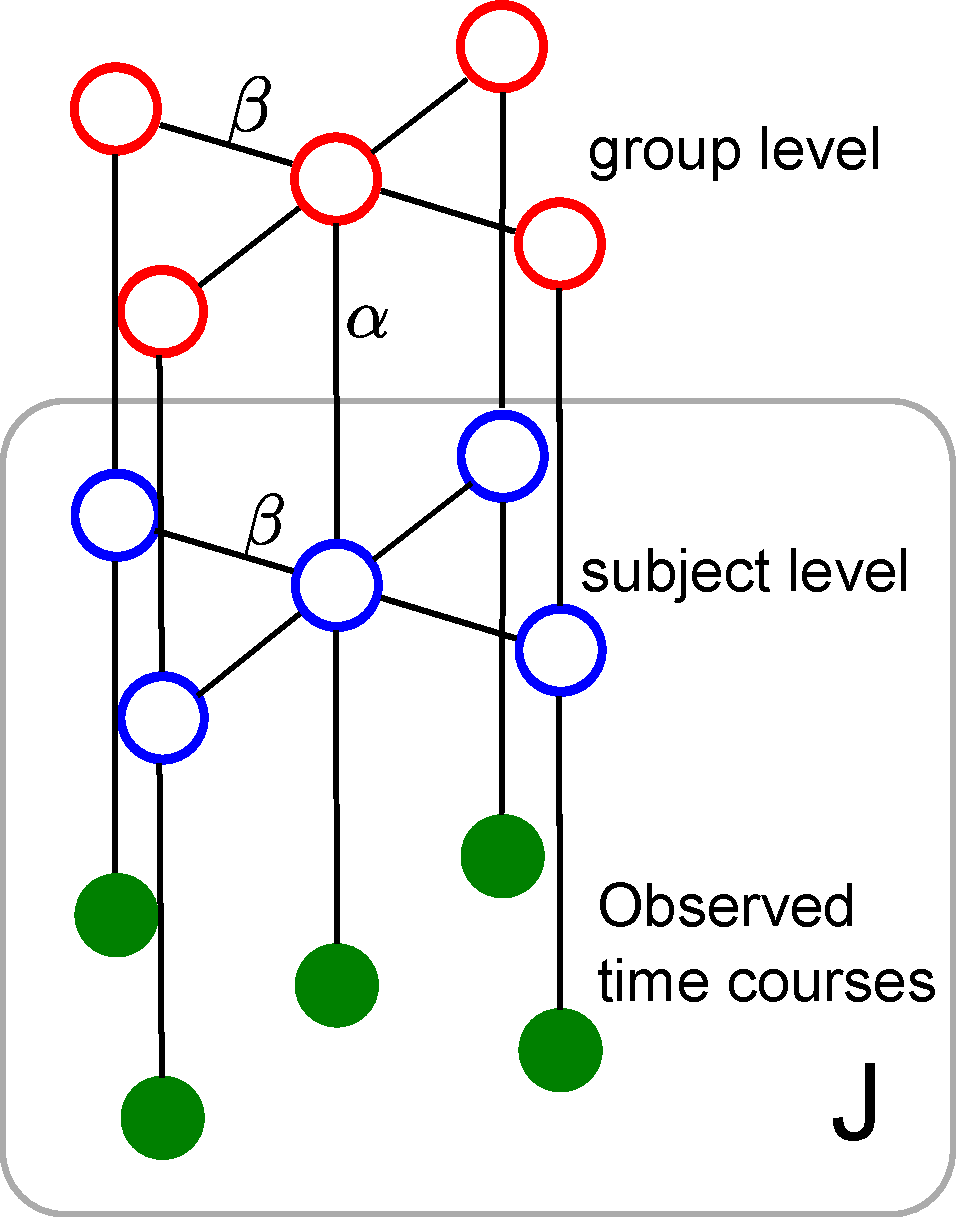
\includegraphics[width=0.4\textwidth]{figures/method3/grp2}
  \caption{We define a MRF on a graph that includes the voxels of all subject
    maps as well as the group map. The set of edges includes the between-level
    links with weight $\alpha$, and within-subject links with weight
    $\beta$. The square box on the subject level and time courses repeats $J$
    times the nodes in the square, representing all the subjects. Only the
    central voxels connection is shown for the between-level links, whereas in
    practice the links exist on all other voxels. The BOLD signal variables
    are shaded, meaning they are set to the observed value.}
  \label{fig:graphical}
\end{figure}

\begin{figure}[]
  \centering
  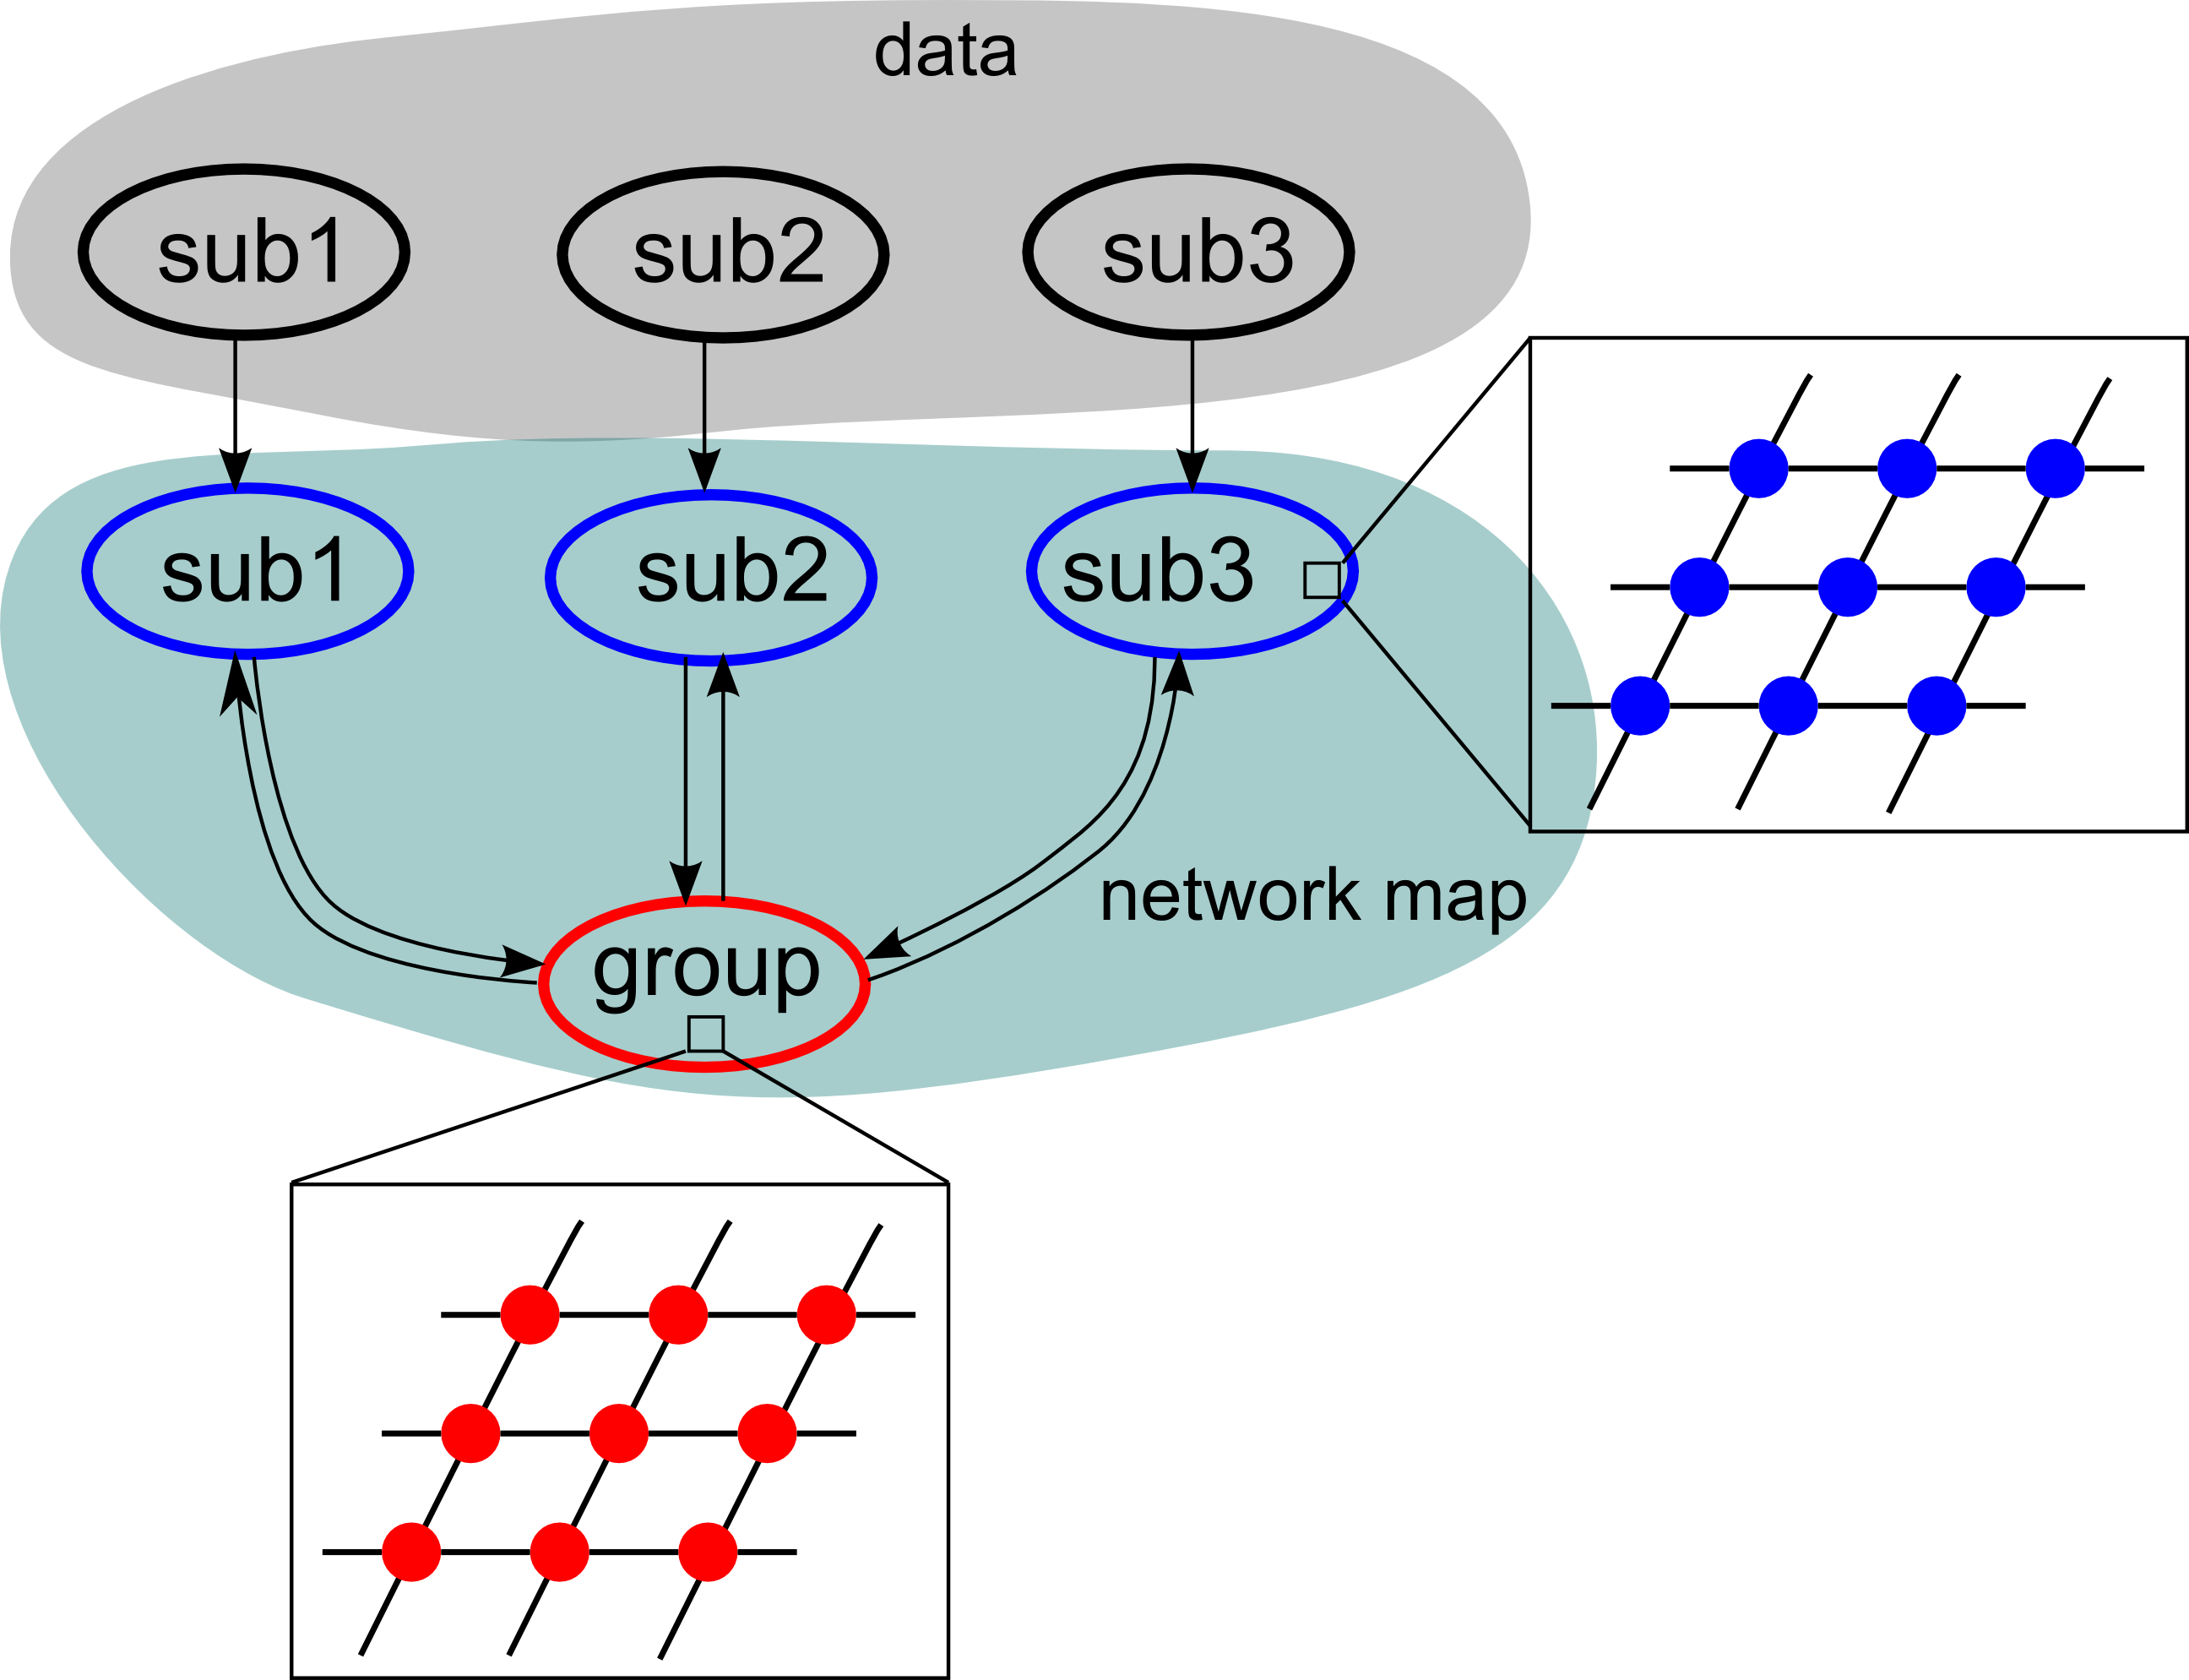
\includegraphics[width=0.5\textwidth]{figures/method3/hier3a}
  \caption{An alternative representation of the graphical model of the HMRF. A
    regular MRF is defined on the network variables within subject, and within
    group label maps. Then between-level links are added between the group
    voxel and each subject voxel at the same anatomical location. The added
    edges, together with the original edges, consist of a new graph which
    integrates two levels of variables. }  
  \label{fig:hier3a}
\end{figure}

\begin{figure}[p]
  \centering
  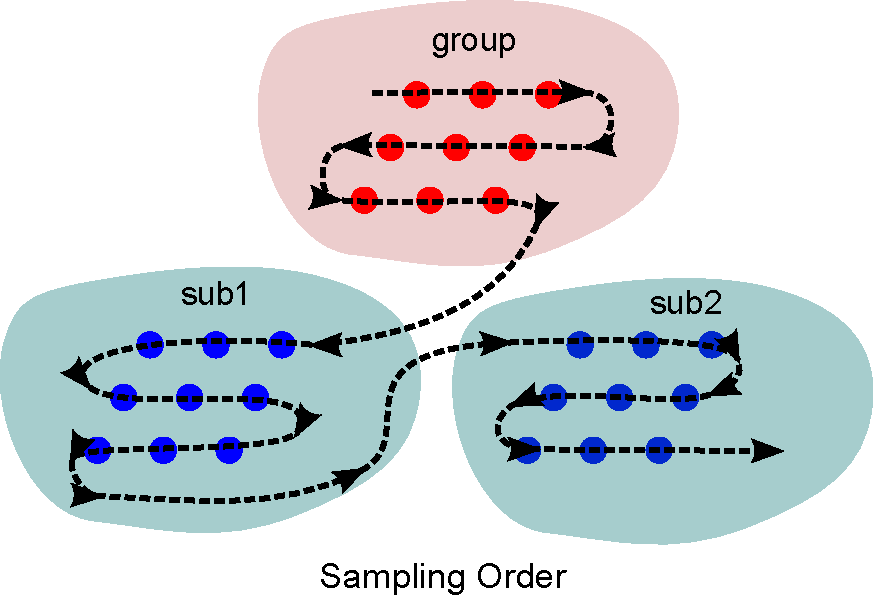
\includegraphics[width=0.5\textwidth]{figures/method3/hiergibbs2}
  \caption{Gibbs sampling schedule on a high level view. The sampling scan of all
    voxels in the group before updating each subject. This schedule repeats until
    convergence.}
  \label{fig:hiergibbs2}
\end{figure}

\begin{figure}[p]
  \centering
  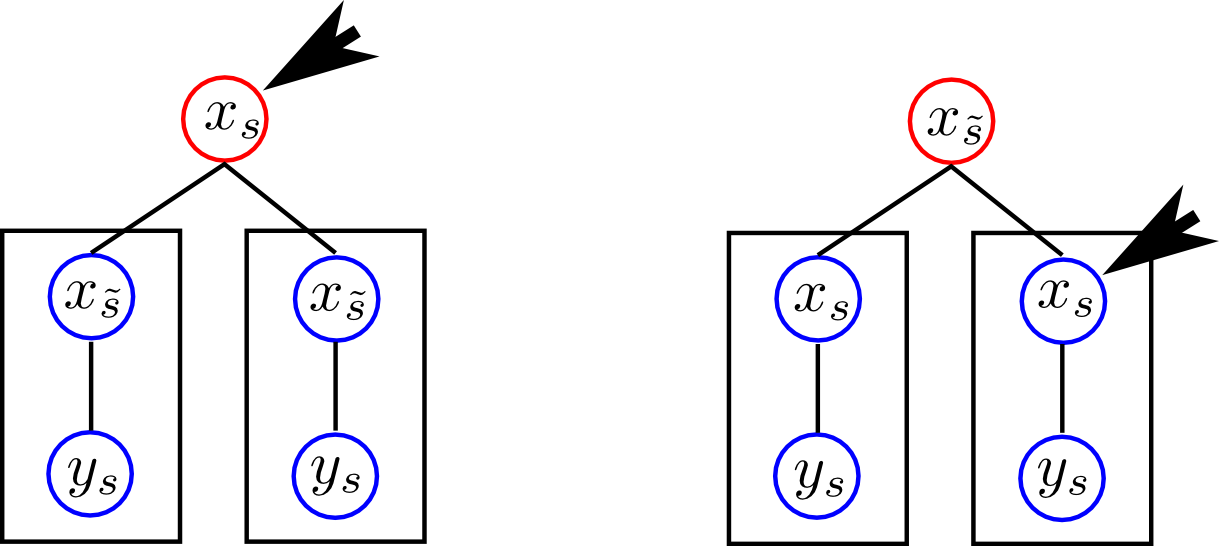
\includegraphics[width=0.5\textwidth]{figures/method3/voxelgibbs}
  \caption{Gibbs sampling iterates between group and subjects. On the
    voxel-level, the sampler draws samples of one voxel given its neighbors that
    includes both with-subject and between-level neighbors. }
  \label{fig:voxelgibbs}
\end{figure}

\begin{figure}[p]
  \centering
  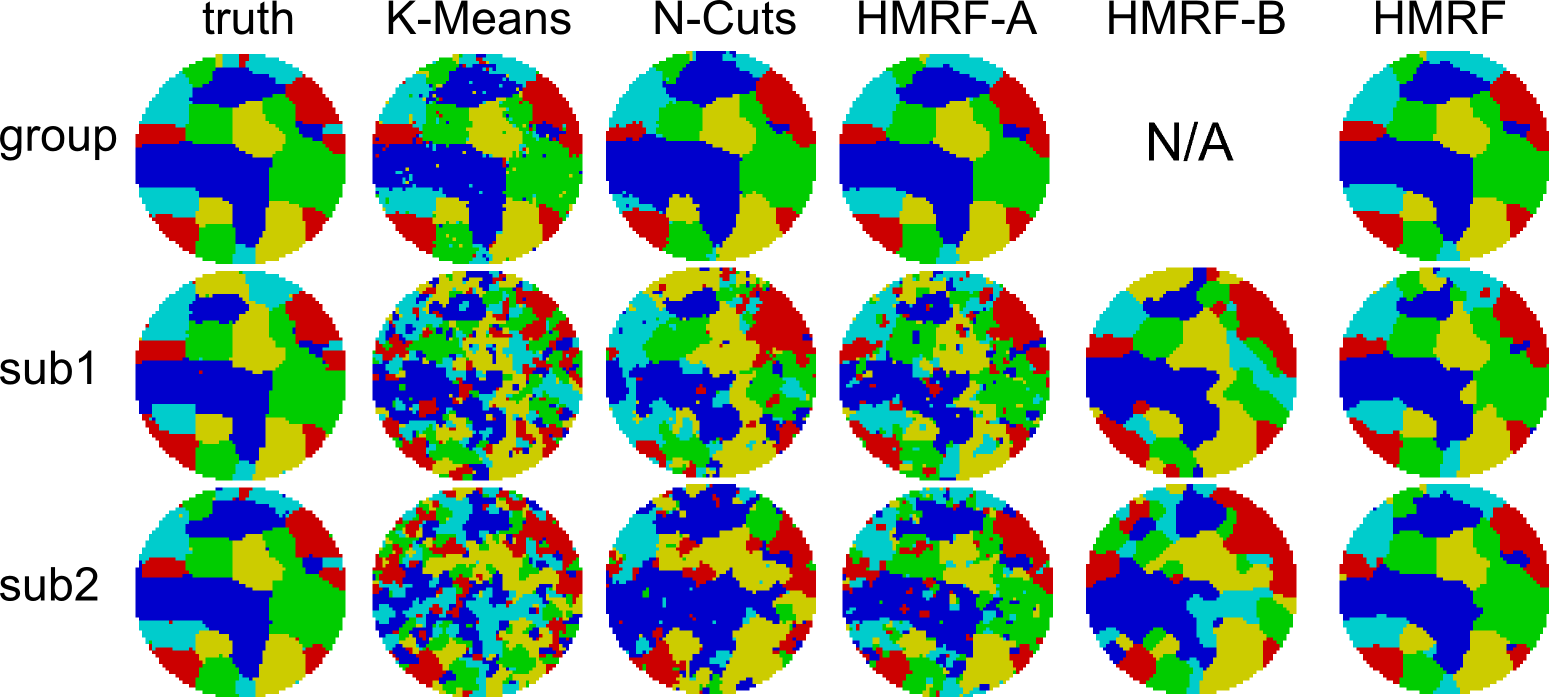
\includegraphics[width=1\textwidth]{figures/method3/allmaps}
  \caption{The estimated group and subject functional network label maps from
    various methods, as well as the ground truth maps. Only two are shown among
    the 25 subjects. }
  \label{fig:synmap}
\end{figure}

\begin{figure}[p]
  \centering
  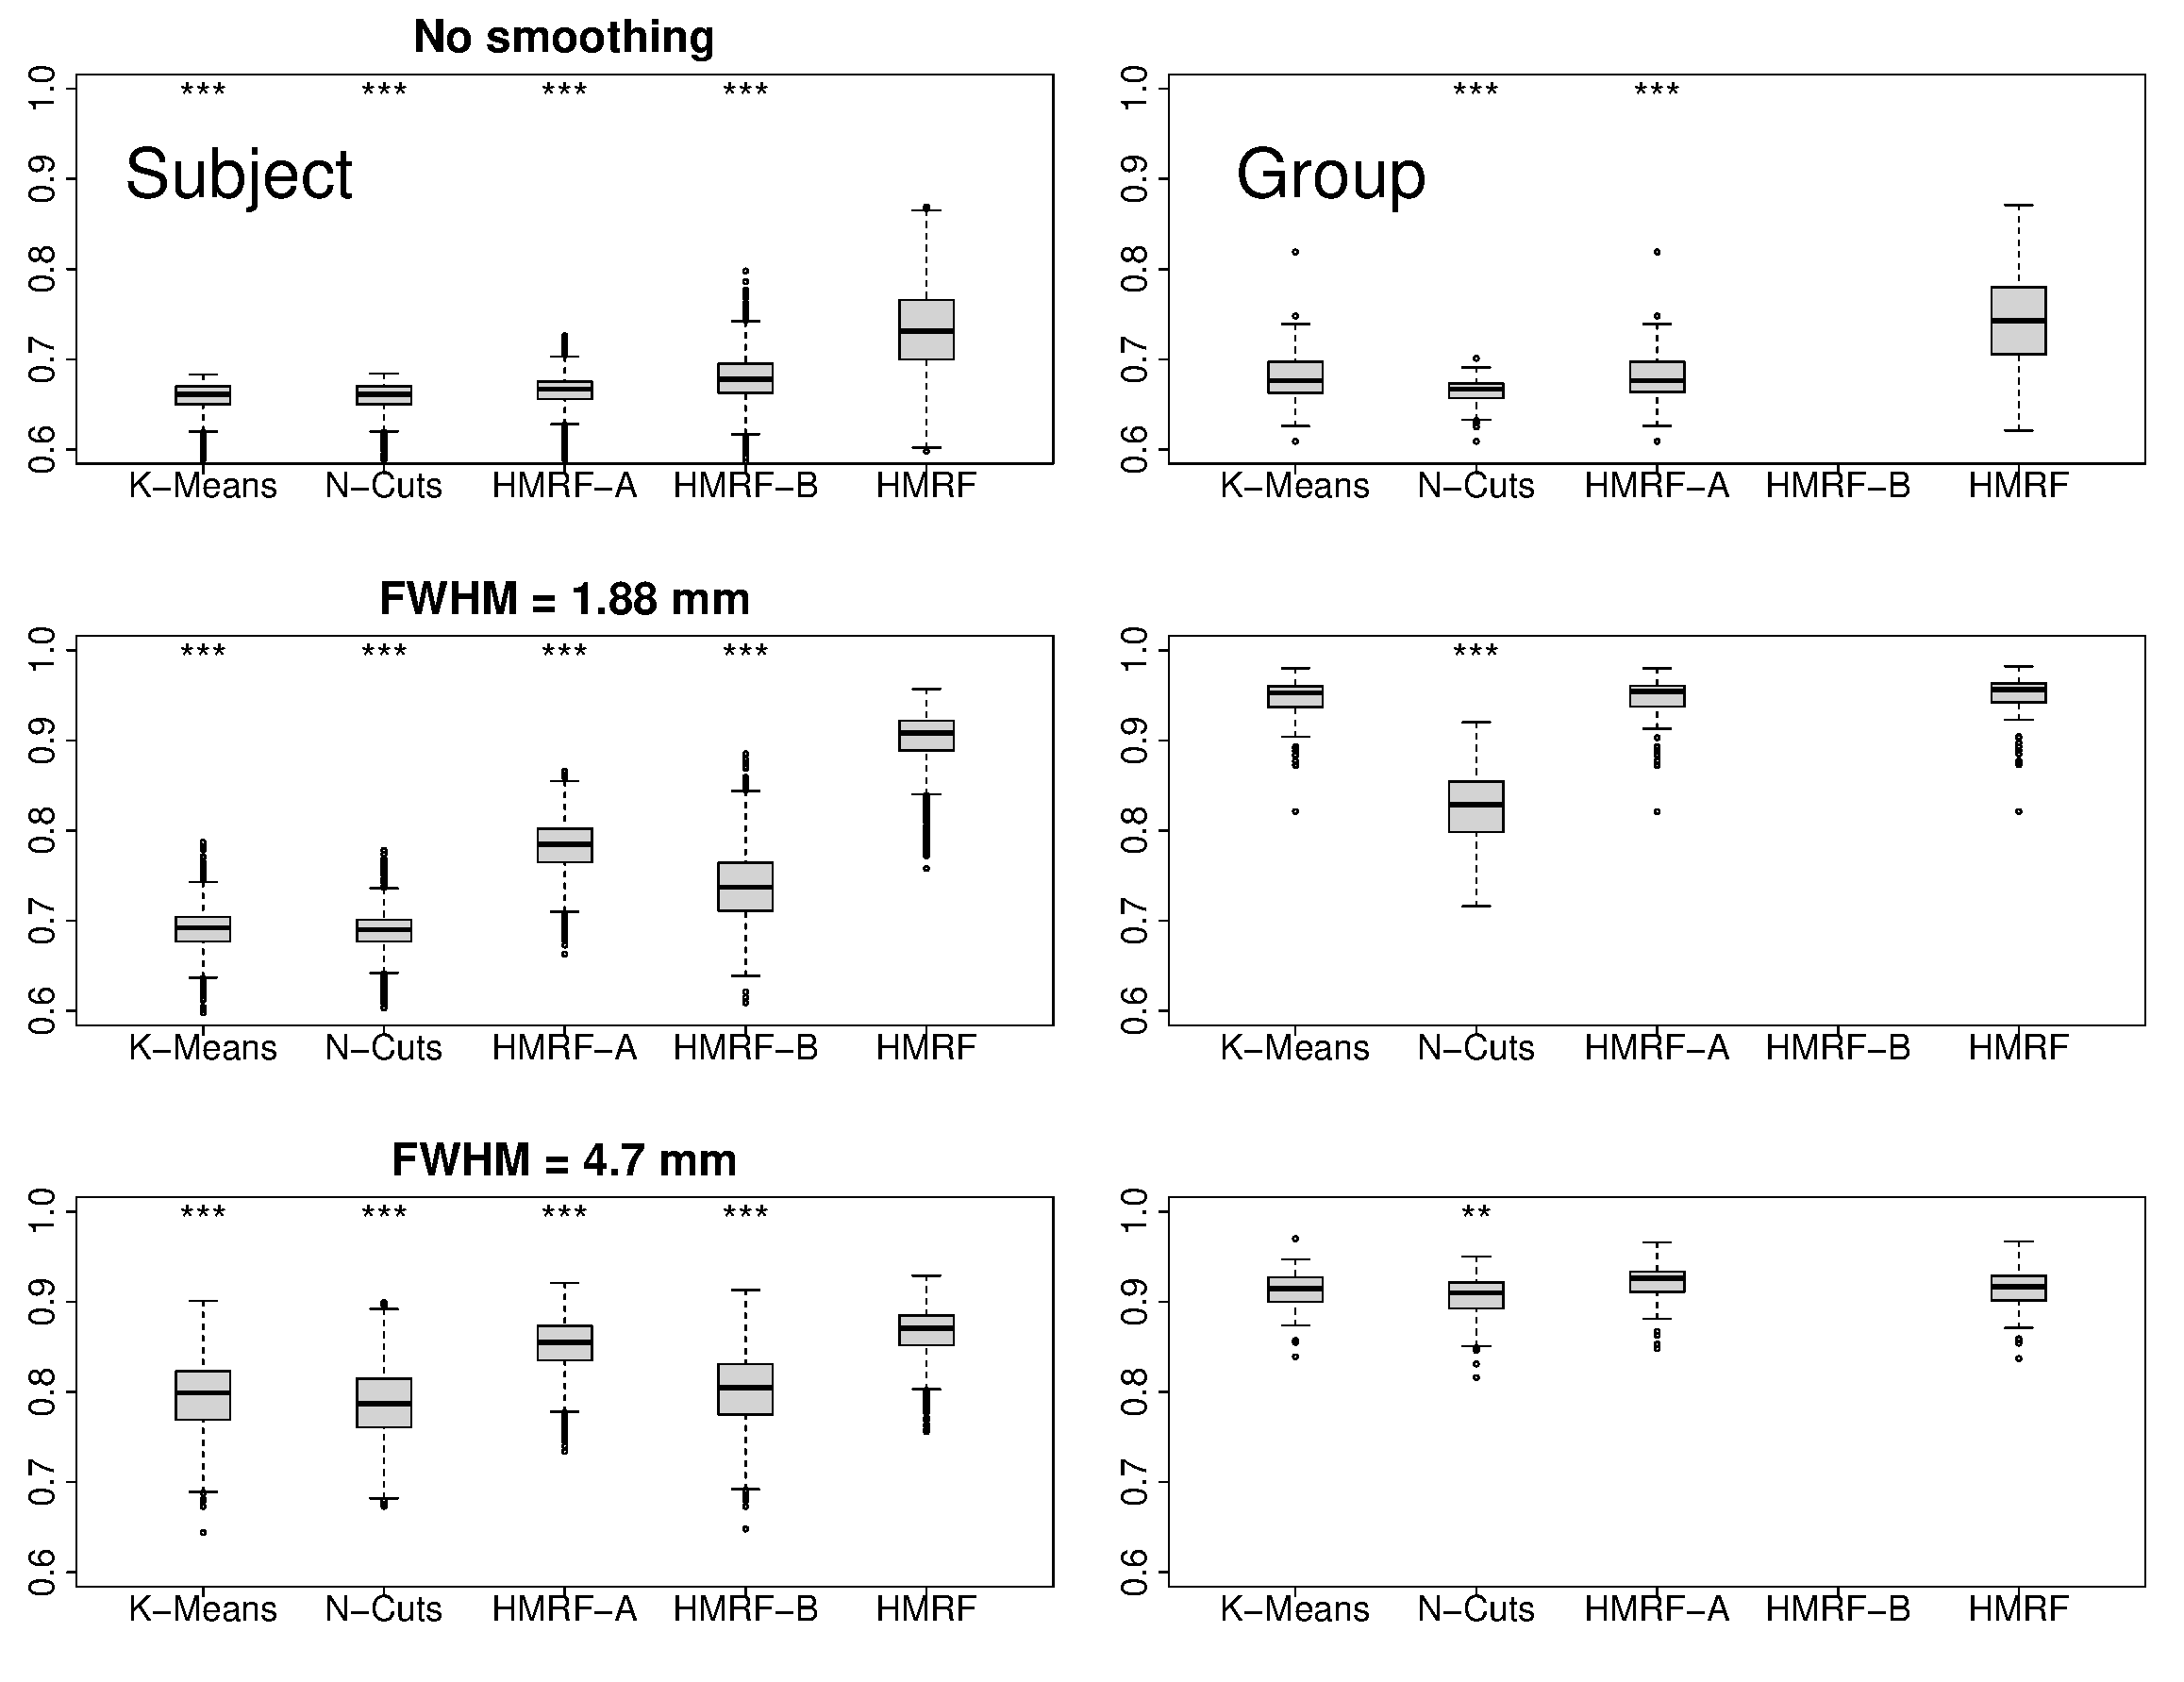
\includegraphics[width=1.0\textwidth]{figures/method3/2level_3smoothing}
  \caption{Box-and-whiskers plots of the estimation accuracies of all methods
    for three levels of spatial smoothing. The accuracies of
    subject labels are across all subjects and MC samples. The group
    map accuracies are across all MC samples. The upper and lower ``hinges''
    correspond to the $25$th and $75$th percentiles. The asterisk on top of each
    box indicates the p-value of the standard two-tailed T test between HMRF and
    the corresponding method. No asterisk: significant $p > 0.05$; $*$:
    significant at $p < 0.05$; $**$: significant at $p < 0.01$; ${***}$:
    significant at $p < 0.001$. The group map is not applicable to HMRF-B due to
    its lack of between-level links.}
  \label{fig:synboxplot}
\end{figure}

\begin{figure}[p]
  \centering
  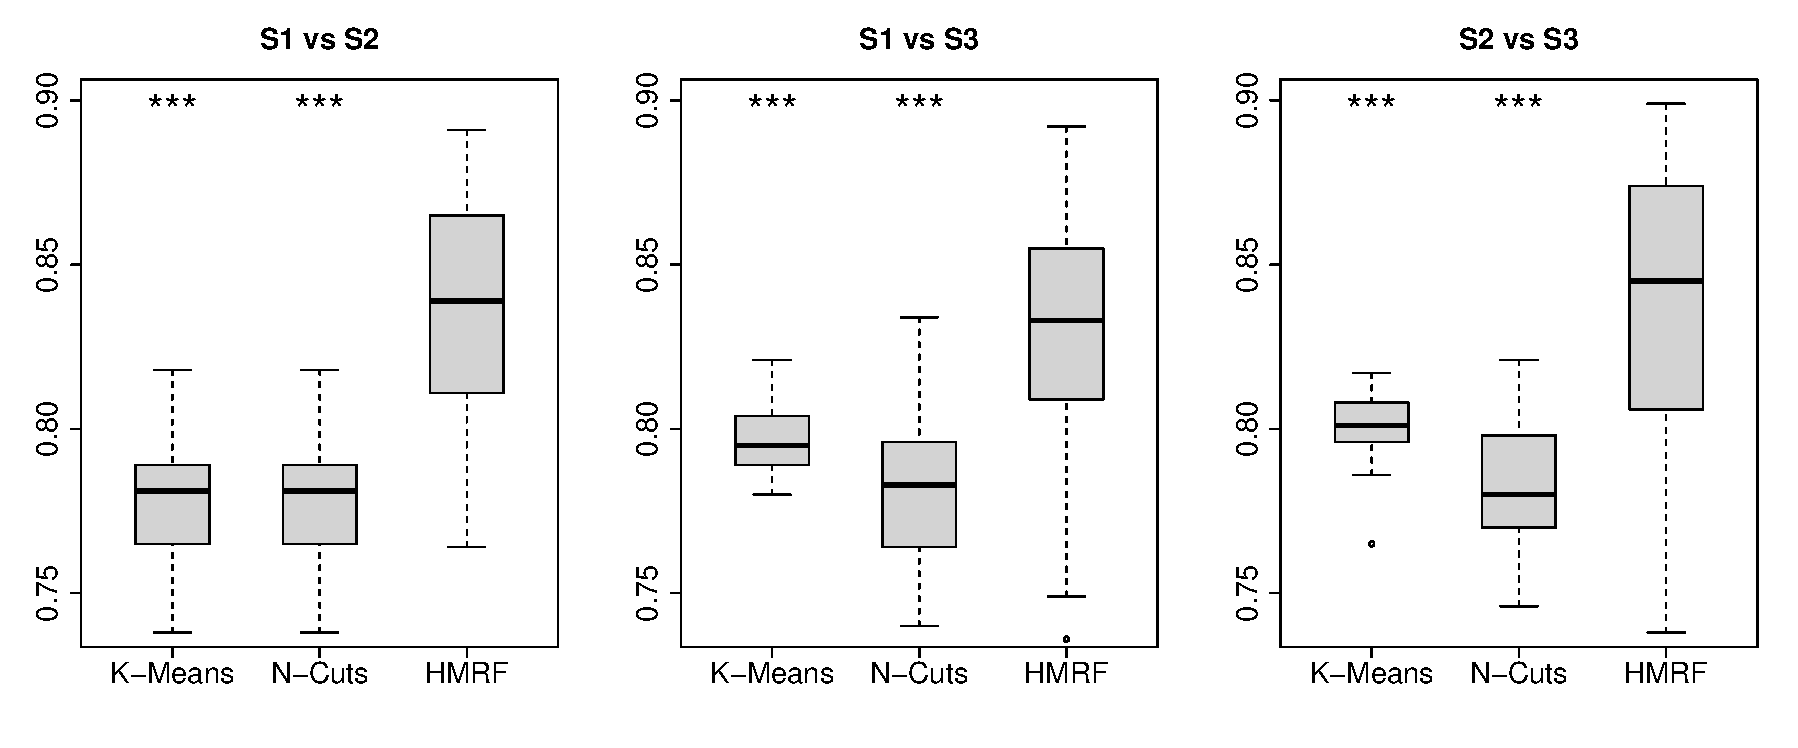
\includegraphics[width=1.0\textwidth]{figures/method3/boxplot}
  \caption{Box-and-whiskers plots of the RI value between each pair of
    sessions over the all subjects' label map. The bottom and top of the boxes are
    the $25$th and $75$th percentile, and the whiskers extend to the whole
    range of the data except the outliers.}
  \label{fig:sessionbox}
\end{figure}

\begin{figure}[p]
  \centering
  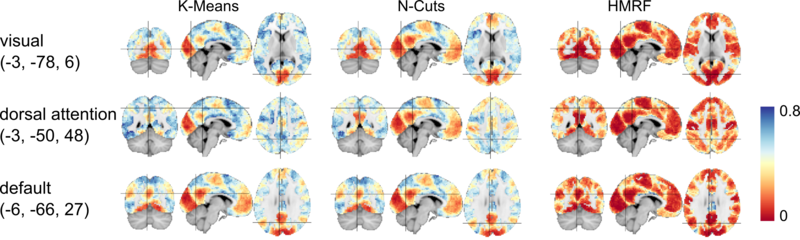
\includegraphics[width=1.0\textwidth]{figures/method3/012variance}
  \caption{The intersession variance maps for three segmentation methods. The
    variance maps are obtained for each subject, averaged across subjects, and
    finally normalized to [0, 1]. A few voxels with intensity above 0.8 are
    rendered the same as those with intensity 0.8. This single map covers all
    seven functional networks, and we selectively show the slices corresponding
    to the three major networks. The image left is the subject's left, and we
    use the same convention in the following figures. }
  \label{fig:intersessionvar}
\end{figure}

\begin{figure}[p]
  \centering
  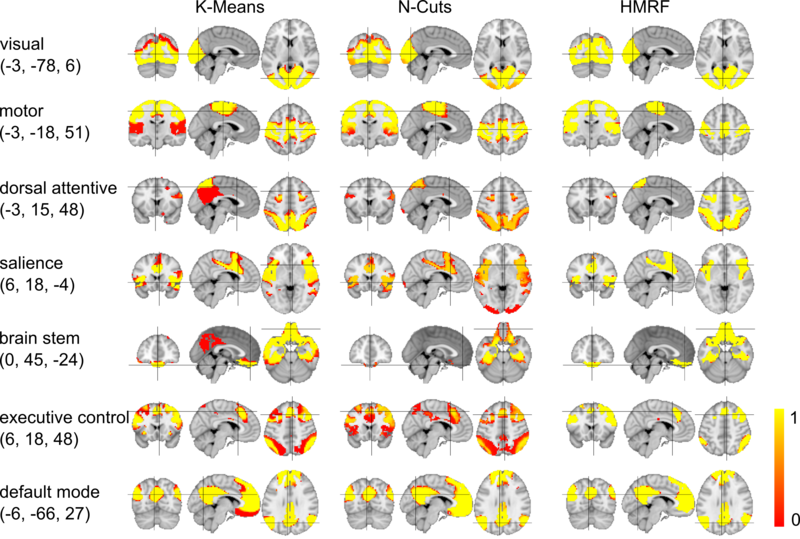
\includegraphics[width=1\textwidth]{figures/method3/grp_mean}
  \caption{The group level's mean functional networks estimated from all
    bootstrapped data by three segmentation methods. The binary map of each
    network is averaged over all bootstrap samples. The average intensity ranges
    from 0 to 1.}
  \label{fig:grpmean}
\end{figure}

\begin{figure}[p]
  \centering
  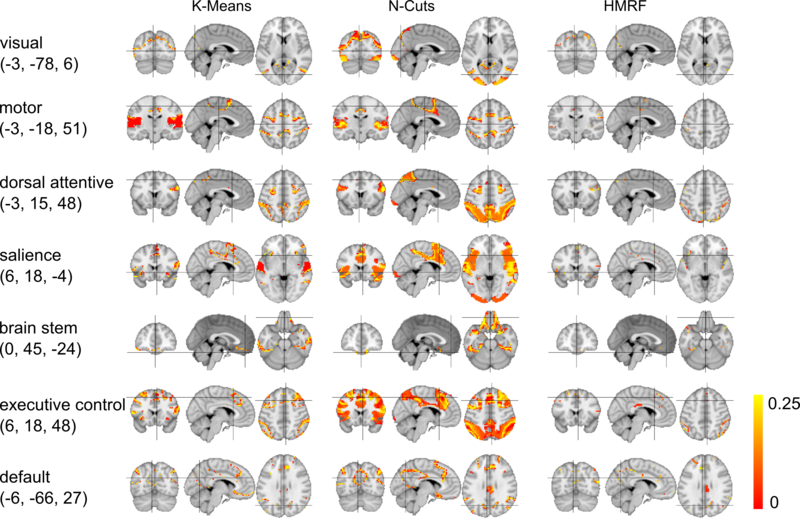
\includegraphics[width=1.0\textwidth]{figures/method3/grp_var}
  \caption{The group variance map estimated from all bootstrap data by the three
    segmentation methods. The variance ranges from 0 to 0.25. }
  \label{fig:grpvar}
\end{figure}

\begin{figure}[p]
  \centering
  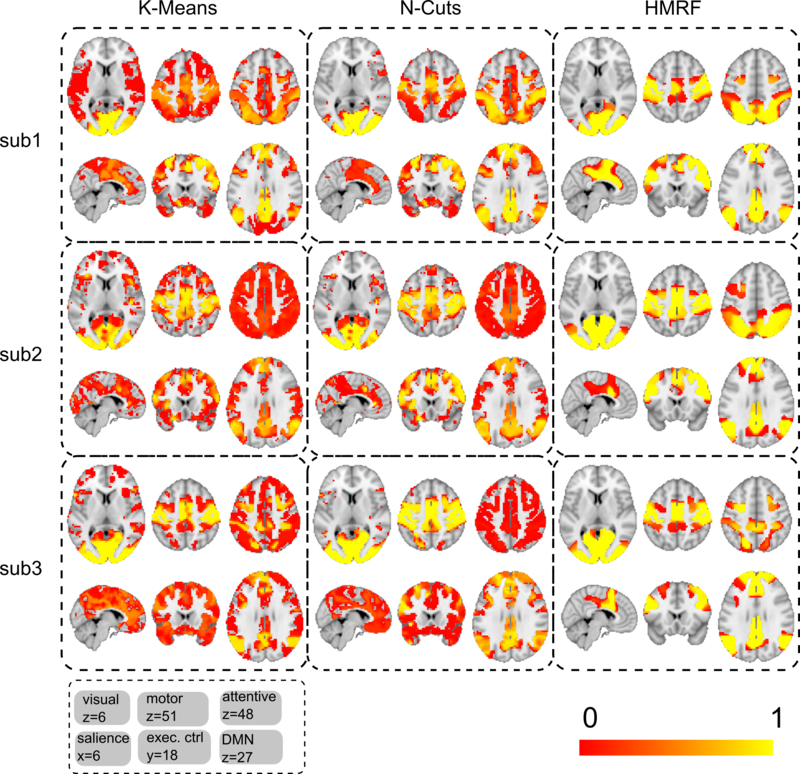
\includegraphics[width=1.0\textwidth]{figures/method3/submean}
  \caption{The three  subjects' average network label maps estimated from all
    bootstrap samples. One representative slice is shown for each of the seven
    networks for each subject (row) and each method (column), excluding brain
    stem component. The average values range from 0 to 1. }
  \label{fig:submean}
\end{figure}

\begin{figure}[p]
  \centering
  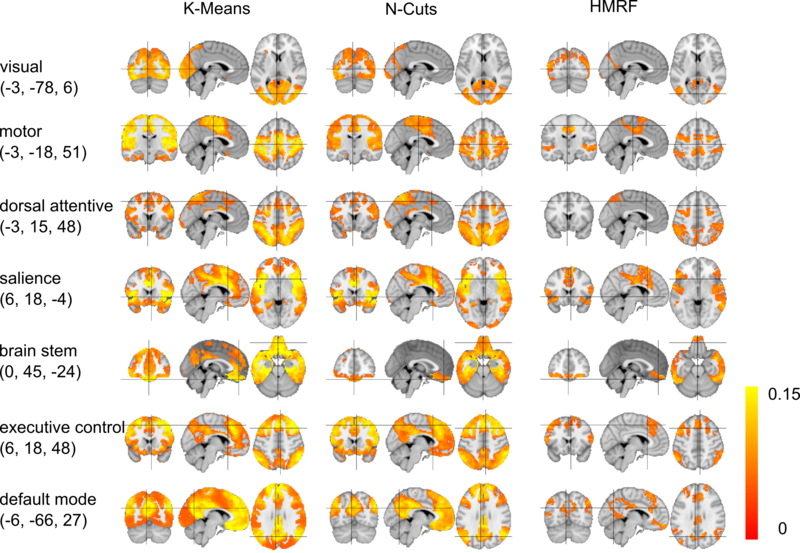
\includegraphics[width=1.0\textwidth]{figures/method3/sub_var}
  \caption{The subjects' variance maps estimated from all bootstrap samples. The
    maps are averaged across all subjects, and their values range from 0 to
    0.25. The color map is in [0, 0.15] since most of the variance values fall
    into this range.}
  \label{fig:subvar}
\end{figure}

\begin{figure}[p]
  \centering
  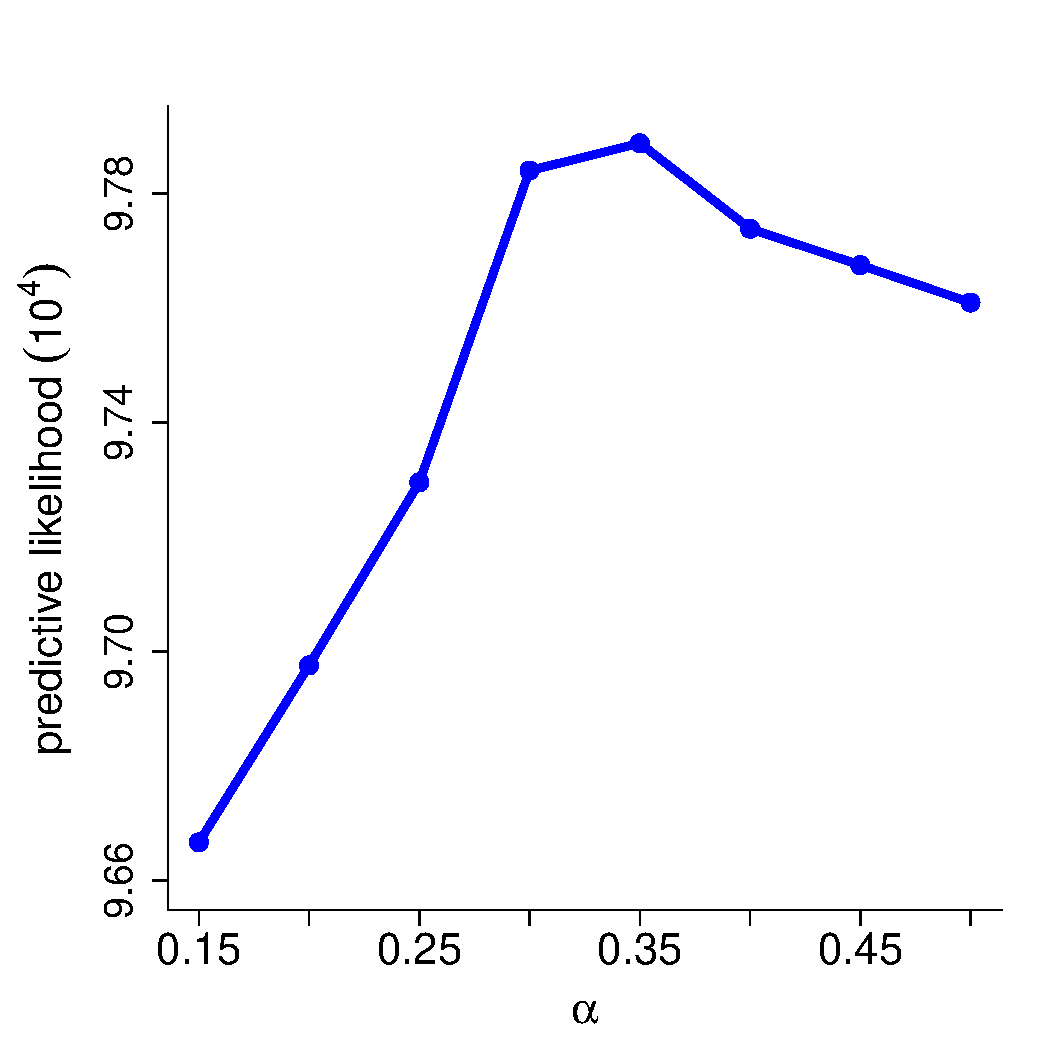
\includegraphics[width=0.5\textwidth]{figures/method3/predictLLvsAlpha}
  \caption{Estimation of parameter $\alpha$ with the average predictive
    distributions using the leave-one-out cross-validation. We use the data from
    only the first session of the NYU-TRT dataset but find similar patterns in
    the other two sessions. $\alpha$ are sampled between 0.15 and 0.5, with
    interval 0.05.}
  \label{fig:alphaest}
\end{figure}

%%% Local Variables: 
%%% TeX-master: "MyThesis"
%%% End: 
